\documentclass[11pt,letterpaper]{article}
\usepackage[utf8]{inputenc}
\usepackage[top=2.54cm,bottom=2.54cm,left=4cm,right=2.5cm,headheight=14pt]{geometry}
\usepackage{graphicx}
\usepackage[hidelinks,bookmarksnumbered]{hyperref}
\usepackage[all]{hypcap}
\usepackage{fancyhdr}
\usepackage[calcwidth]{titlesec}
\usepackage{chngcntr}
\usepackage{booktabs}
\usepackage[dvipsnames]{xcolor}
\usepackage{listings}
\usepackage[section]{placeins}
\usepackage[style=iso]{datetime2}
\usepackage{pgf-umlsd}
\usepackage{amsmath}
\usepackage{cite}
\usepackage[nottoc,numbib]{tocbibind}
\usepackage{comment}
\usepackage{pgfgantt}
\usepackage{todonotes}
\usepackage{ragged2e}
\usepackage{textcomp}
\usepackage{array}
\usepackage{pdflscape}

\title{BioSense Wearable}
\author{Samuel Dewan, Tadhg Mcdonald-Jensen, Jason Nyentap, and Morgan Smith}

% Headers and footers
\pagestyle{fancy}
\fancyhf{}
\lhead{Final Report}
\rhead{BioSense Wearable}
\rfoot{\thepage}

% More space around figures
\setlength\intextsep{18pt}
% Per section figure and table numbers
\counterwithin{figure}{section}
\counterwithin{table}{section}

% Colour links rather than putting a box around them
\hypersetup{
    colorlinks,
    linkcolor={black},
    citecolor={blue!50!black},
    urlcolor={blue!80!black},
    pdftitle={Project 21}
}

% More space between table rows
\renewcommand{\arraystretch}{1.2}

% Section numbers in the margin
\newcommand{\marginsecnumber}[1]{%
    \makebox[0pt][r]{#1\hspace{6pt}}%
}
\titleformat{\section}
    {\sffamily\Large\bfseries}
    {\marginsecnumber\thesection}
    {0pt}
    {}
\titleformat{\subsection}
    {\sffamily\large\bfseries}
    {\marginsecnumber\thesubsection}
    {0pt}
    {}
\titleformat{\subsubsection}
    {\sffamily\normalsize\bfseries}
    {\marginsecnumber\thesubsubsection}
    {0pt}
    {}

% Draft watermark
\usepackage{eso-pic,graphicx}
\AddToShipoutPicture*{%
    \AtTextCenter{%
        \makebox(0,0)[c]{\resizebox{\textwidth}{!}{%
        \rotatebox{45}{\textsf{\textbf{\color{lightgray}DRAFT}}}}}
    }
}

\begin{document}
\frenchspacing

% Title Page
\pagenumbering{Alph}
\begin{titlepage}
\centering

\vspace*{\stretch{1}}
{\large \textbf{SYSC4907}}

\vspace{\stretch{1}}
{\Huge \sffamily Final Report}

\vspace{\stretch{1}}
{\large \textbf{BioSense Wearable}}

\vspace{\stretch{1}}
\textbf{Project Group 21}

\vspace{\stretch{0.5}}
Samuel Dewan

{\footnotesize 101041496}

{\footnotesize samueldewan@cmail.carleton.ca}

Tadhg McDonald-Jensen

{\footnotesize 101047069}

{\footnotesize tadhgmcdonaldjensen@cmail.carleton.ca}

Jason Nyentap

{\footnotesize 101032473}

{\footnotesize jasonnyentap@cmail.carleton.ca}

Morgan Smith

{\footnotesize 101031075}

{\footnotesize morgansmith@cmail.carleton.ca}

\vspace{\stretch{0.5}}
Supervisor: Dr. Paulo Garcia

\vspace{\stretch{2}}

{\large \textbf{\today}}

\vspace{\stretch{2}}

\end{titlepage}

% Front matter
\pagenumbering{Roman}

%\section*{Abstract}
%\label{sec:abstract}
%Early detection of illness could limit the spread of infection, save lives, and
save money.  One possible method of early detection is to continuously measure
someones physiological state.  Here we detail our creation of such a continuous
biometric measurement device.  The device is in the form factor of a watch and
contains sensors to measure skin temperature, ambient temperature, motion, 
heart rate, pulse oximetry, and UV light. The software drivers for UV light,
heart rate and pulse oximetry were not completed in time so data is only
recorded from motion and temperature sensors. The PCB also supports an air
quality sensor which was never populated due to a lack of availability.
The device is powered by a lithium ion battery that is charged
through a USB port and lasts two days of normal operation.  
The total cost of the unit is \costofboard.  Sensor data can be
obtained through the SD card, USB port, or Bluetooth by using the appropriate companion
software.  The companion software can then produce graphs to display the output
of the sensors.  The focus of this solution is on the collection of biometrics
and making them available for analysis.  No attempt was made to perform medical
analysis or give clinical diagnosis from the collected biometrics.  Our
intention was to design an open source system so that those applications could be
integrated with or built on top of the work we have done for this project.

%\clearpage

\tableofcontents
\clearpage

% Proposal Content
\pagenumbering{arabic}

\section{Overview}
\label{sec:overview}
This section provides an overview of the problem this project aims to solve,
why it is important, how this project can be part of the solution, and finally 
a brief description of what progress was actually made towards the solving the 
problem. Subsequent sections of this report cover the hardware and software design 
of the project in detail, as well as discuss some of the challenges that
were faced in pursuing the solution outlined here. Information regarding the
tests performed on the final project are also detailed in this report, and a
series of appendices are included with visuals to show some interesting parts 
of the design and what the final product looks like.

\subsection{Background}

Traditionally, people only seek treatment for ailments after they start
experiencing symptoms; however, it is often desirable to take action before
symptoms appear.  One solution to catch illness earlier could be to monitor a
person's physiological state using various sensors and take action when the
state falls outside of a known healthy state.  However, the accepted healthy
range for a population could be significantly larger than the accepted healthy
range for the individual \cite{Wearable-tracking2017}.

Wearables are capable of revealing personal daily physiological cycles with
respect to skin temperature, and heart rate with high accuracy
\cite{Wearable-tracking2017}. By comparing a person's current physiological
state with the expected state, it is possible to predict illness with greater
sensitivity than a self diagnosis. For example, a study was able to detect a
period of inflammation (confirmed by a medical high-sensitivity C-reactive
protein test) using a participant's heart rate even though the participant
themselves experienced no symptoms \cite{Wearable-tracking2017}.  The same
study even helped a participant get treatment of Lyme disease before the
``Bull's eye'' rash appeared (a common symptom during the early stages of Lyme
disease) by detecting an abnormality in their SpO\textsubscript{2} levels.

Wearable data can also be used to detect group illness rates.  By using heart
rate data and sleep data from fitbit devices and cross referencing that data
with the Centers for Disease Control and Prevention's (CDC) Influenze Like
Illness (ILI) data, a study was able to predict illness 6.3\% to 32.9\% better
than previous methods \cite{Radin2020}.

Wearables can also detect more immediate dangers to someone's health like a
heart attack \cite{heart-attack}, a fall \cite{Khojasteh_2018}, or dangerously
low or high heart rates.  This information could be used to alert emergency
services to save lives.

\subsection{Motivation}

Despite all of the advances in medical technology, a cure for diseases and
allowing humans to live longer are ever present goals for scientists and 
doctors alike.  Often wide spread diseases we have not prepared for can occur in
society.  COVID-19 is a pandemic that
has, at the time of writing, claimed an estimated 1 million lives globally
\cite{johns-hopkins-corona-chan}, and continues to infect more people every
day.  In 2007 it was estimated that the total cost of occupational illnesses
among civilians in the United States was \$58 billion \cite{Leigh2011}.
Slowing the spread of disease could save lives and save money.

One method of limiting the spread of disease is early diagnosis.  This would
allow individuals who are aware they are ill to take measures to reduce the
spread of their illness, even before symptoms manifest.  This will be
particularly useful for healthcare providers who work with high risk
individuals, since identifying symptoms early has the highest efficiency for
protecting others.

By creating a personal physiological profile and constantly
comparing the user's current physiological state to it, illness can be detected
early.  The motivation for our project is to create a device capable of measuring 
enough of the user's current physiological state to predict illness.  This is done 
in the hope that it could be used to slow the spread of illness's and, to speed
recovery from illness's by starting treatment earlier.

\subsection{Problem Statement}

One way to facilitate early diagnosis is to measure biometrics on patients and
make clinical diagnoses based on these measurements.
A convienient and low cost method to collect biometric data is needed in order
to make the potential benefits of the technology available to a large number of
people. This information may then be used to detect abnormalities in the user’s 
physiology and could be used to aid in the early detection of illness.
The objective of this project is to create a wearable device that can measure a
variety of critical health metrics including skin temperature and heart rate.

\subsection{Solution}

The solution provided by this project is a wrist mounted wearable health 
monitoring device. The device provides a sensor platform that is suitable for 
early detection of disease. The included sensors can measure skin temperature, 
ambient temperature, heart rate, pulse oximetry, and motion.  The electronic
components fit into a comfortable, wearable 3D printed plastic enclosure.
The device is powered by a lithium polymer battery which can be recharged
through the USB-C connector.

The wearable device has limited user interfaces consisting of an indicator
LED for power, notifications, and debugging. It also features a power button
to turn the device on and off. The main interactions with the device occur 
through a companion software that connects to the device through Bluetooth or 
USB. It is limited to simply receiving and decoding data received from the 
wearable device, and exporting it in an analyzable format such as a csv or json 
file.

The device will store the collected sensor information to a micro SD card
in the device which is then read back when requested via the companion software.
The SD card will be replaceable, and the capacity of the card used will dictate
how long the device can record data before needing to off load to the companion
software.

The focus of this solution is on the collection of biometrics and making them
available for analysis. No attempt was made to perform medical analysis
or give clinical diagnosis from the collected biometrics. Our intention was to
design the system so that those applications could be integrated with or built
on top of the work we have done for this project.

\subsection{Accomplishments}
{\color{red}
What did we actually do?
}

%Should this be in a reflection or something? Not really part of a solution,
%it is a disclaimer.

%In order to reduce development cost and complexity, the hardware component of
%the project uses sensors that are readily available from online sources, and 
%that can be assembled on a PCB by hand relatively easily. As a result the 
%selection of sensors may be more limited or lower quality than what is possible 
%if options that are made to order, or only available in large quantities had been
%explored.  The use of parts that can be soldered to a PCB without paying for
%the services of an advanced manufacturing facility also resulted in the final 
%hardware design being larger than it would have been otherwise.

\clearpage

\section{Engineering}
\label{sec:engineering}
\subsection{Health and Safety}
% {\color{red}
% Using the Health and Safety Guide posted on the course webpage, students will 
% use this section to explain how they addressed the issues of safety and health 
% in the system that they built for their project.
% }
Due to Covid restrictions all electrical work was performed without supervision.  
Since all electrical work uses USB power of 5V no risk of serious injury was possible.
To mitigate risk of shock, it was ensured that work area is clear and that there are no live wires exposed while the board is connected to the power source.
All soldering was performed within reasonable safety guidelines.

\subsection{Engineering Professionalism}
% {\color{red}
% Using their course experience of ECOR 4995 Professional Practice, students 
% should demonstrate how their professional responsibilities were met by the 
% goals of their project and/or during the performance of their project.
% }
% Several aspects of the project were affected by engineering practices
In order to ensure user privacy is maintained, the data collected by the device is only stored locally and
can only be offloaded by USB (physical access) or over bluetooth using standard bluetooth encryption.
The device is enclosed in a way that ensures that electrical shock is not possible under normal operation.
The bluetooth module we are using is industry canada certified to be safe to use.

\subsection{Project Management}
% {\color{red}
% One of the goals of the engineering project is real experience in working on a 
% long-term team project. Students should explain what project management 
% techniques or processes were used to coordinate, manage and perform their project.
% }
Each member of the team was, due to individual passions, interested in different
aspects of the project, thus division of tasks was organic and did not require a leader or dictating division of work.
Good communication over instant messaging and occasional meetings to discuss updates and re-evaluating
task assignment ensured fair distribution and completion of work.
Though we had created a timeline,
due to underestimating the amount of time certain tasks would take to
accomplish, the timeline had to be pushed back. Working with a group and
deadlines enabled the development of time management skills.


\subsection{Justification of Suitability for Degree Program}

All team members are studying Computer Systems Engineering.  This program
teaches hardware, software, and the intersection between them.  This gave us a
strong foundation for developing our project as an embedded system.  We
applied what we have learned in ELEC and SYSC courses related to embedded
processors to develop our own hardware platform.  This required us to
exercise our electronic circuit analysis skills using concepts like Ohms law or
Kirchhoff’s voltage and current laws to make sure our electronics work
properly.  In order to connect all of our sensors and interfaces to the
embedded processor we used what we have learned about microcontroller
peripherals such as UART, I2C, SPI, GPIO, and timer modules.  In addition to 
creating our own hardware, we wrote software that runs on the embedded processor
to control the device.  The C programming language was used to do this, and we 
applied much of the knowledge and techniques learned from several SYSC courses.  
This includes concepts like interrupts, managing multiple tasks and events, 
using the hardware features of the embedded processor and more.  Some of the
non-technical courses included in the Computer Systems Engineering program have 
also proved useful for managing the project and writing reports. 
% this final sentence is weird.
Since we 
have applied large portions of the knowledge gained from our studies to
out project we believe the project is relevant to what we have studied and 
relevant to our degree program.
% due to the previous courses taken by members of the group, we feel as though we can apply our theoretical knowledge to a practical application more efficiently

\subsection{Individual Contributions}
In this section, the contributions of each group member to the project are
presented. The contributions are divided into those related to the project 
itself, and secondly those related to the writing of this report.

\subsubsection{Project Contributions}
The list below details the contributions of each group member towards the
implementation and testing of the project. In cases where components were 
shared by group members, percentages are given.

\begin{itemize}
    \item Hardware component research and selection - Jason 50\%, Sam 50\%
    \item Electronic prototyping - Jason
    \item Schematic capture - Jason 80\%, Sam 20\%
    \item PCB layout - Jason
    \item PCB assembly - Sam
    \item Hardware Debugging - Sam
    \item Bill of materials and Purchasing - Sam
    \item Command line interface - Sam
    \item USB driver - Sam
    \item Analog interface code - Sam
    \item ICM 20948 IMU driver - Sam
    \item Data logging and file systems - Sam
    \item Bluetooth driver - Jason
    \item Bluetooth interface for companion software - Jason 60\%, Tadhg 40\%
    \item Companion app CLI interactions and usb connection - Tadhg
    \item log file parsing and plotting - Tadhg
    \item Companion app automated testing - Tadhg
    \item Enclosure design - Morgan
    \item Enclosure fabrication - Morgan
    \item MAX86150 PPG/ECG driver - Morgan
    \item Guix package - Morgan
    \item SI1133 UV light sensor driver - Tadhg
\end{itemize}

\subsubsection{Report Contributions}
The list below details the contributions of each group member towards this final
report. In cases where sections were shared by group members, percentages are
given.

\begin{itemize}
    \item 0 Abstract - Morgan
    \item 1.1 Motivation - Morgan 50\%, Tadhg 50\%
    \item 1.2 Problem Statement - Jason
    \item 1.3 Solution - Tadhg
    \item 1.4 Accomplishments - Morgan
    \item 1.5 Report Structure - Tadhg
    \item 2.1 Health and Safety - Tadhg
    \item 2.2 Engineering Professionalism - Tadhg
    \item 2.3 Project Management - Tadhg
    \item 2.4 Justification of Suitability for Degree Program - Jason
    \item 3 State of the Art - Jason
    \item 4.1 Component Selection - Sam 80\%, Jason 20\%
    \item 4.2 Schematic - Jason
    \item 4.3 PCB Layout - Jason
    \item 4.4 Enclosure - Morgan
    \item 5 Software Implementation Description - Sam
    \item 5.4.1 USB - Sam
    \item 5.4.2 Bluetooth - Jason
    \item 5.4.3 Heart Rate - Morgan
    \item 6.1 Integration Testing - Sam
    \item 6.2 Performance Measurements - Sam
    \item 6.3 Power Measurements - Jason
    \item 6.4 Companion App Testing - Tadhg
    \item 6.5 Physical Dimensions - Morgan
    \item 6.6 Cost - Sam
    \item 7.1.1 Power and Battery Design Challenges - Jason
    \item 7.1.2 Assembly and Parts Availability Challenges - Sam
    \item 7.2.1 Toolchain and nRF5 SDK Challenges - Sam
    \item 7.2.2 USB and Bluetooth Integration Challenges - Jason
    \item 8 Timeline - Morgan
    \item 9 Conclusion - Tadhg
\end{itemize}

\clearpage

\section{State of the Art}
\label{sec:state-of-the-art}
Wearable health monitoring devices have been progressing in areas including
form factor, biometric data collection, and battery life.  This section will
discuss the current state of commercially available solutions, as well as some
ongoing research areas.

Commercially available wearable health monitoring devices come in a variety of
different form factors depending on their intended use and their capabilities.
These include wrist-mounted devices such as smartwatches and wrist bands,
head-mounted devices, straps, textiles, and various
others \cite{Seneviratne2017}.  The type of device most relevant to this
proposal is the wrist band.  They may be equipped with a selection of sensors
and a processor, but have no display.  An example of such a device is the Empatica
E4 wristband \cite{McCarthy2016}.  This device is designed to provide real-time
physiological data for research using a photoplethysmogram, electrodermal
activity sensor, accelerometer, and temperature sensor \cite{empatica}. The
device can log data internally, stream it over Bluetooth, and has an API for
developing smartphone apps that make use of the data it collects. Empatica
claims that their device has been used by researchers in over 1000 studies
\cite{empatica}.

Many modern wearable health monitoring devices offer a similar suite of sensors
that measure heart rate, temperature, motion, and more
\cite{Seneviratne2017}.  A novel type of sensor that has yet to be incorporated
into these devices is a sweat sensor.  Sweat sensors are chemical sensors that
can non-invasively analyze the user's sweat at a molecular level in order to
detect biomarkers.  If sweat is not produced naturally, they can induce
sweating to facilitate measurements \cite{Tai2018}.  One of the limitations on
the number and type of sensors that can be put in a wearable device is their
location, since some sensors require specific placement on the
body \cite{Baig2017}.  A workaround for this is to use textile sensors.  If the
wearable device is a long sleeve shirt for example, then it can cover the arms,
chest, and back all at once.  This allows for more freedom in sensor placement
than what is allowed by a wrist band.  Nanomaterial sensors are being developed
that can be placed either directly on skin or made into textiles that can be
worn.  Many sensors can be made using this technology including temperature
sensors, strain rate sensors, tactile sensors, electrophysiological sensors,
electrochemical sensors, and more \cite{Yai2018}.

Like smart-phones or other mobile devices, powering wearable health monitoring
devices can be a challenge \cite{Pantelopoulos2010}.  Longer battery life is 
desirable but usually comes at the cost of weight and size.  
Wearable devices place yet another constraint on this problem: comfort 
\cite{Motti2014}.  Comfort enables users to wear the device continuously for 
long periods of time.  

One way of overcoming the battery problem is through the use of 
specialized textiles that can generate or store electricity.  Triboelectric 
nanogenerator fabric can be used to generate electricity from the movement of 
the person wearing it, and that energy can be stored in another fabric which 
is made with supercapacitor yarn.  This energy can then be used by the 
electronics of the wearable device \cite{Pu2016}.  Another method of generating 
electricity from the wearer of the device is to take advantage of body heat.  
This can be done using wearable thermoelectric power generators that are flexible 
and conform to the area of the body they are attached to.  They rely on a 
temperature difference between the ambient air and the surface they are attached 
to in order to generate electricity \cite{Siddique2017}.  Wearable devices that 
rely on batteries can also take advantage of specialized textiles.  Zinc ion 
batteries have been made into film that is both flexible and safe in the case 
of impact, puncture, and washing \cite{Li2018}.

A contrasting approach to reducing the battery capacity requirement of wearable 
devices is power conservation.  Dynamic power consumption of electronic 
components is related to their supply voltage, capacitance, and operating 
frequency \cite{Forman1994}. All three of these factors can be reduced in order 
to save power.  Supply voltage can be reduced by using components designed to 
operate on lower voltages, capacitance can be reduced by using highly integrated 
components or multichip modules, and frequency can be reduced by lowering 
processor clock speeds at the cost of performance \cite{Forman1994}.  An
additional benefit of highly integrated electronics for wearable devices is 
there can be fewer components required in the hardware design, leading to 
a smaller final product.  An embedded processor in a wearable device could make 
use of an adjustable clock, or multiple clock sources in order to slow the 
processor down when high performance is not needed to conserve power.  Even
when high performance is needed certain tasks can be offloaded to dedicated
hardware that is more efficient, thus allowing the processor to remain in a 
lower power state.  AES encryption for example has been shown to have lower 
power consumption and increased performance when dedicated hardware is used
instead of a software implementation \cite{Hamalainen2006}.  For this reason,
wearable devices using encryption for communication or data storage may 
benefit from using a processor with hardware cryptography support. Another task
directly related to wearable devices that has seen benefit from hardware 
acceleration is real time ECG signal processing \cite{Cardarilli2018}. It was 
shown that hardware acceleration allowed for a reduction in processor clock 
speed without sacrificing execution time, resulting in significant power 
savings.

By combining the power generation, storage, and conservation technologies 
aforementioned, it may be possible to create future wearable health monitoring 
devices that are just as comfortable to wear as regular clothing, never 
require charging, and are essentially maintenance-free for the life of the unit.

In summary, it appears that significant research and development has gone into
moving wearable health monitoring devices away from the current design of a
battery-powered device affixed to the body in some way, and towards comfortable
textiles that cover the body, monitor biometrics, and power themselves from the
body.  Unfortunately, the technology required for these desirable qualities is 
not yet mature enough to be inexpensive and readily available.  As a result,
the wearable device this project aims to create will have to be more in line 
with some of the commercially available products out there today. It is
possible however to apply some of the power conservation techniques using 
technology available today. Hardware acceleration and higher levels of 
integration can be achieved using embedded processors with several built in
modules for things like Bluetooth, USB, cryptography, and more. There are also
sensors available that integrate measurement of several different parameters 
and may even perform some signal processing all in a single chip. Many 
opportunities exist for a wearable device to slow down or stop its processor in
order to save power, such as between sensor readings, or when not interacting
with the user. All of these technologies, constraints and possibilities are 
important considerations when designing a wearable health monitoring device.

\clearpage

\section{Hardware Implementation}
\label{sec:hardware}
This section will describe the hardware component of the project and explain 
the rationale for some important design decisions including component selection,
schematic design, and component placement on the PCB. It will also detail any 
variations from what was planned in the project proposal and why these changes
were made.

\subsection{Component Selection}

A number of requirements were considered in choosing a microcontroller for our
project. We identified several microcontroller features that were required to
meet our project requirements and omitted any microcontrollers
without these features from consideration. These features include:
\begin{itemize}
    \item Bluetooth Low Energy support
    \item At least one I2C master mode interface for sensors
    \item An SPI or SD/MMC interface to connect and SD card
\end{itemize}

We chose to limit our selection of microcontrollers to those that included parts 
that featured an integrated Bluetooth LE radio. This is
to reduce part count (and therefore size, cost and design complexity) and to
provide better power consumption.

Table \ref{tab:mcu-comp-general} shows a brief summary of the microcontroller
options that we considered, all of which met the minimum criteria outlined
above. The costs listed in the table are in Canadian dollars in single
quantities from digikey.ca. Different prices are compared, as they may vary.

All of the parts listed are based on ARM cortex processors. Nordic
Semiconductor's nRF5340 and the Silicon Labs’ EFR32BG22C224 use a Cortex-M33
while all other listed microcontrollers use a Cortex-M4. We estimated that
any of these microcontrollers would have sufficient processor performance for
our application. Similarly, all of the listed options have ample flash storage
and SRAM.

Not all of the listed microcontrollers come in packages that are easy to solder
by hand. The relatively small QFN packages of the nRF52832 and EFR32BG22C224 can
be soldered with relative ease using a hot air reflow station or an iron and be
inspected easily with a microscope. Unfortunately the other options are much
more difficult, as the Apollo3 Blue's BGA package and the WLP package of the
MAX32668 each have a large array of solder balls. These packages can be soldered
with hot air reflow, but we did not have the equipment to inspect them. The
nRF52840 and nRF5340 are a middle ground, their aQFN packages have many fewer
balls, but they still do have two rows of connections. This means that while we
are able to solder the packages with hot air reflow they would also be difficult to
inspect. Another option that was considered to bypass the issue of soldering 
difficulty was the use of modules that integrate the microcontroller and
a PCB antenna on a small PCB. The nRF52840 and nRF52830 can be found in these
modules and the Apollo3 Blue is available in a similar module from SparkFun as SparkFun Artemis.

Availability was also a limiting factor in our decision. Most of our listed
microcontrollers were readily available from a variety of online
vendors. The exception was the Apollo3 Blue, which was not readily available
outside of SparkFun's Artemis module, and the MAX32668 which is a newly
available part and could only be ordered as a sample from Maxim's
website.

\begin{table*}[htb]
\centering
\begin{tabular}{>{\centering\arraybackslash}m{2.2cm}|
                >{\centering\arraybackslash}m{2.5cm}|
                >{\centering\arraybackslash}m{2.0cm}|
                >{\centering\arraybackslash}m{1.5cm}|
                >{\centering\arraybackslash}m{1.2cm}|
                >{\centering\arraybackslash}m{1.8cm}|
                >{\centering\arraybackslash}m{1.2cm}}
\toprule
Part Number & Manufacturer & CPU & Program Memory & SRAM & Friendliest Package & Cost \\
\midrule
nRF52840 & Nordic Semiconductor & ARM Cortex-M4 at 64 MHz & 1 MiB & 256 KiB  & aQFN73 & \$9.34 \\
nRF52832 & Nordic Semiconductor & ARM Cortex-M4 at 64 MHz & 512 KiB & 64 KiB  & QFN48 & \$8.19 \\
nRF5340 & Nordic Semiconductor & Dual ARM Cortex-M33 at 96/64 MHz & 1 MiB & 512 KiB & aQFN94 & \$13.85 \\
Apollo3 Blue & Ambiq & ARM Cortex-M4 at 48 MHz & 1 MiB & 384 KiB & BGA81 & N/A \\
MAX32668 & Maxim Integrated & ARM Cortex-M4 at 96 MHz & 1 MiB & 560 KiB & WLP109 & N/A \\
EFR32BG22 C224 & Silicon Labs & ARM Cortex-M33 at 76.8 MHz & 512 KiB & 32 KiB & QFN40 & \$5.26 \\
\bottomrule
\end{tabular}
\caption{Comparison of Microcontrollers With Bluetooth Low Energy Radios}
\label{tab:mcu-comp-general}
\end{table*}

Table \ref{tab:mcu-comp-comm} compares the communications interfaces available
on the microcontrollers under consideration. All microcontrollers feature at
least Bluetooth Low Energy 5.0, at least two I2C interfaces and at least two SPI
interfaces. In addition to these interfaces the MAX32668 has an SD/MMC interface
controller which supports the SD3.0 specification. This interface would allow
significantly faster SD card access speeds than we can accomplish using an SPI
interface.

The nRF52840 and MAX32688 both feature USB interfaces. We decided to have a USB
CDC-ACM interface for debugging and as a wired alternative to the
Bluetooth interface for data transfer. While we could have implemented a USB
interface with any of the microcontrollers listed by using a separate USB to
UART chip, using one of the microcontrollers with a built-in USB interface 
gives us greater integration saving us cost, board space, complexity and
power usage.

\begin{table*}[htb]
\centering
\begin{tabular}{>{\centering\arraybackslash}m{3.0cm}|
                >{\centering\arraybackslash}m{1.8cm}|
                >{\centering\arraybackslash}m{1.8cm}|
                >{\centering\arraybackslash}m{1.8cm}|
                >{\centering\arraybackslash}m{1.5cm}|
                >{\centering\arraybackslash}m{3.0cm}}
\toprule
Part Number & I2C Master Interfaces & SPI Master Interfaces & SD/MMC Interface & BLE Version & USB \\
\midrule
nRF52840 & 2 & 4 & None & 5.2  & 2.0 Full Speed \\
nRF52832 & 2 & 3 & None & 5.2  & None \\
nRF5340 & 4 & 5 & None & 5.1 & None \\
Apollo3 Blue & 6 & 6 & None & 5.0 & None \\
MAX32668 & 3 & 3 & SD3.0 & 5.0 & 2.0 High Speed \\
EFR32BG22C224 & 2 & 2 & None & 5.2 & None \\
\bottomrule
\end{tabular}
\caption{Comparison of Microcontroller Communications Hardware}
\label{tab:mcu-comp-comm}
\end{table*}

While our project did not necessarily require hardware accelerated cryptography,
we thought it should be included to accommodate any future software layers that
build on top of our platform. Since the device collects information about the
user, it is likely that cryptography would be heavily used by security features so
software implementations of the cryptographic algorithms may not be adequate.
Table \ref{tab:mcu-comp-crypto} shows the cryptography features of the
microcontrollers that we considered. All of the microcontrollers have suitable
hardware accelerated cryptography features with the exception of the nRF52832
which lacks modular arithmetic acceleration for public key cryptography and
the Apollo3 Blue which has no hardware cryptography accelerator.

\begin{table*}[htb]
\centering
\begin{tabular}{>{\centering\arraybackslash}m{2.5cm}|
                >{\centering\arraybackslash}m{2.0cm}|
                >{\centering\arraybackslash}m{2.0cm}|
                >{\centering\arraybackslash}m{2.5cm}|
                >{\centering\arraybackslash}m{2.5cm}|
                >{\centering\arraybackslash}m{1.5cm}}
\toprule
Part Number & Hashes & Public Key Algorithms & Symmetric Key Algorithms & AES Modes & True Random Number Generator \\
\midrule
nRF52840 & SHA-1, SHA-2 up to 256 bits, HMAC & RSA up to 2048 bit key, ECC & AES128, ChaCha20, Poly1305 & ECB, CBC, CMAC/CBC-MAC, CTR, CCM/CCM* & Yes \\
nRF52832 & None & None & AES128 & ECB, CCM & No \\
nRF5340 & SHA-1, SHA-1 up to 256 bits, HMAC & RSA up to 3072 bit key, ECC & AES128, AES256 & ECB, CBC, CMAC/CBC-MAC, CTR, CCM/CCM*, GCM & Yes \\
Apollo3 Blue & None & None & None & None & No \\
MAX32668 & SHA-2 up to 512 bits & RSA up to 4096 bit key, ECC & AES128, AES192, AES256, DES, 3DES & ECB, CBC, CFB, OFB, CTR & Yes \\
EFR32BG22 C224 & SHA-1, SHA-2 up to 256 bits & ECC & AES128, AES192, AES256 & ECB, CTR, CBC, CFB, GCM, CBC-MAC, GMAC, CCM & Yes \\
\bottomrule
\end{tabular}
\caption{Comparison of Microcontroller Cryptography Hardware}
\label{tab:mcu-comp-crypto}
\end{table*}

Because of its availability, easy to work with package, suitable
serial interface, integrated USB support and hardware cryptography acceleration,
we chose to use the nRF52840 microcontroller. While the Apollo3 Blue had low 
power features, it had questionable availability and a complete lack of hardware 
accelerated cryptography. The MAX32668 would also have been a very good 
option, but it is not yet widely available. The EFR32BG33C224 was excluded due to the lack of an 
integrated USB interface and comparatively little documentation.
More specifically, it was decided to use a module (BMD-340) containing the
nRF52840 instead of just chip itself. This was because 
the module is much more readily available, has a built in Bluetooth 
antenna already been certified by several different parties, is 
easier to solder, and includes several supporting components for the 
microcontroller, such as oscillators and capacitors. While the module is more 
expensive and larger than the microcontroller by itself, it is more cost-effective due to
the additional components it contains.

The selection of sensors that made it into the final design are an inertial 
measurement unit (IMU), a heart rate sensor, an air quality sensor, a UV light 
sensor, an infrared temperature sensor and an ambient temperature sensor. This 
suite of sensors was selected in order to capture as much information as 
possible without increasing the cost of the device too much. The 
choice of each of these sensors was mostly driven by cost, availability, and 
ease of soldering. The infrared temperature sensor and ambient temperature 
sensor are both integrated into the same component. The ambient temperature 
sensor will indicate the temperature of the user’s environment while the 
infrared temperature sensor measures the user’s body temperature. The air 
quality sensor and UV light sensor will provide additional information about 
the user’s environment. The IMU will provide information about the user’s 
movements, and the heart rate sensor will measure the user’s heart rate. A 
listing of the exact components used for each of these sensors is provided 
below.

\begin{itemize}
   \item ICM-20948: Inertial Measurement Unit (IMU)
   \item MAX86150EFF+T: Heart rate sensor
   \item ZTP-148SR: Infrared and ambient temperature sensor
   \item BME680: Air quality sensor
   \item SI1133-AA00-GM: UV light sensor
\end{itemize}

\subsection{Schematic}

The schematic is split into three major sections; the power supply, 
processor, and sensors. The power supply is responsible for managing the 
devices internal lithium-ion polymer (LiPo) battery and powering all other 
parts of the circuit. When the device’s USB-C port is connected to a 
suitable host, the power supply will shift the electrical load from the 
internal battery to the USB power source and begin charging the internal 
battery. When USB power is disconnected, charging stops and the electrical load is 
shifted back to the internal battery. Transitions between the two power 
sources are seamless and will not interrupt operation of the 
device. Upon request by the processor, the power supply can also perform fast 
charging of the battery. The processor is responsible for communicating with 
all onboard sensors and the internal SD card through several I2C and SPI 
buses. Communication with the outside world is also handled by the processor
through the USB-C port or wirelessly over Bluetooth. The collection of onboard 
sensors is responsible for gathering information about the user and their 
environment to be used by the processor.

The implementation of the power supply was mostly guided by the remaining system requirements and cost. 
The majority of the components in the design 
require 1.8V to operate, with exceptions being the RGB status LED and the SD 
card, requiring 3.3V. The status LED does not have a specific voltage 
requirement, but 1.8V was not sufficient to overcome the forward voltage of the 
diodes so 3.3V was used instead with appropriate series current limiting 
resistors. The choice of a LiPo battery meant that the power supply input 
voltage could be anywhere from 3.7V to 2.8V depending on state of charge, and 
when connected to USB power the input would be 5V. There were several ideas on 
how to build a power supply that would meet all the requirements, but the final 
decision is pictured in Figure \ref{fig:BlockDiagram_PowerSupply} as a block 
diagram.

\begin{figure}[!htb]
\centering
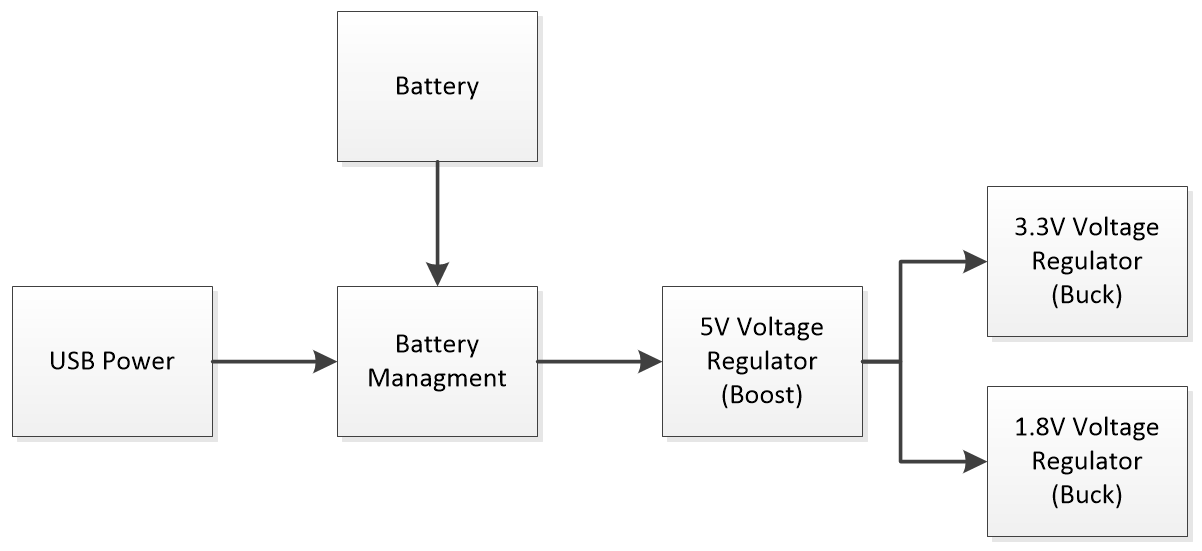
\includegraphics[width=\textwidth]{images/BlockDiagram_PowerSupply.png}
\caption{Block diagram of power supply.}
\label{fig:BlockDiagram_PowerSupply}
\end{figure}

The battery and USB power input are both connected directly to a dedicated 
battery management IC. This IC handles battery charging, battery protection,
%you need to define what IC stands for and use brackets when defining it (isomething csomething (IC)) 
and automatic switchover from one power source to the other. It does not 
however provide any means of regulation. Regulation is handled by three 
separate voltage regulators, the first of which boosts the input up to 5V. The 
last two regulators step the output of the 5V regulator down to 3.3V and 1.8V. 
The intermediate 5V is not strictly necessary as 5V is not used anywhere in the 
design, but without it the 3.3V regulator would need to be a more expensive 
buck-boost type since the input voltage could be above or below its output. 
Additionally, the 5V regulator has an enable input that is used in conjunction 
with some soft power on/off circuitry to completely isolate the load from the 
power source and reduce standby power consumption to nearly zero. Another option 
that was considered was using the voltage regulator built into the chosen 
processor to generate the 1.8V from 3.3V. Due to concerns over robustness and maximum current limitations, the latter option was rejected. 
With the current design, both the 3.3V and 1.8V regulators can operate independently of 
each other, have short circuit protection with automatic recovery, have overheating 
protection, can deliver much more current than needed, and should 
operate with over 90\% efficiency according to the device datasheets. The result 
is a very robust, safe, and cheap solution that integrates well with the rest of 
the design.

One interesting design feature related to the power supply is the way in which 
the device is powered on and off. The most obvious approach was to use a simple 
on/off switch that connects or disconnects power from the load, but some flaws 
were identified with this idea; suddenly removing power from the microcontroller 
during writes to the SD card or communication over USB or Bluetooth may cause 
data corruption. Also, if the battery is allowed to die completely with the 
switch left on, the device may “flicker” on and off. The next obvious approach was to leave power permanently 
connected to the microcontroller and use a momentary push button to toggle 
between a very low power state and normal operation. This solution solves the 
data corruption problem but does not eliminate the possibility of power 
“flicker” with a dead battery, and also suffers from unnecessarily high standby 
power consumption since the device does not actually turn off. Elements of both 
approaches were used to come up with a design that solves all of these problems. 
When the device is off, the power source and load are completely isolated by 
disabling the 5V regulator, depicted in Figure \ref{fig:BlockDiagram_PowerSupply}. 
A momentary power button enables this regulator when pressed, turning on the 
device. As soon as the microcontroller starts up it uses one of its GPIO pins to 
latch the power supply on before the user releases the momentary button. The 
momentary button and GPIO pin are the inputs to a logical OR gate that controls 
the enable pin of the voltage regulator. This means that the device will stay 
powered up for as long as the microcontroller desires regardless of what the 
user does with the power button. A separate signal from the momentary button is 
routed to an input pin of the microcontroller so that it can determine when the 
user presses the button. If the user holds down the button for an extended period 
of time the microcontroller will go through a shutdown routine, ending with turning 
off the GPIO pin that latched the power supply on. As soon as the user releases 
the power button all power will be lost and the device is now off. A simplified 
schematic view of this arrangement is depicted in 
Figure \ref{fig:BlockDiagram_OnOff} below.

\begin{figure}[!htb]
\centering
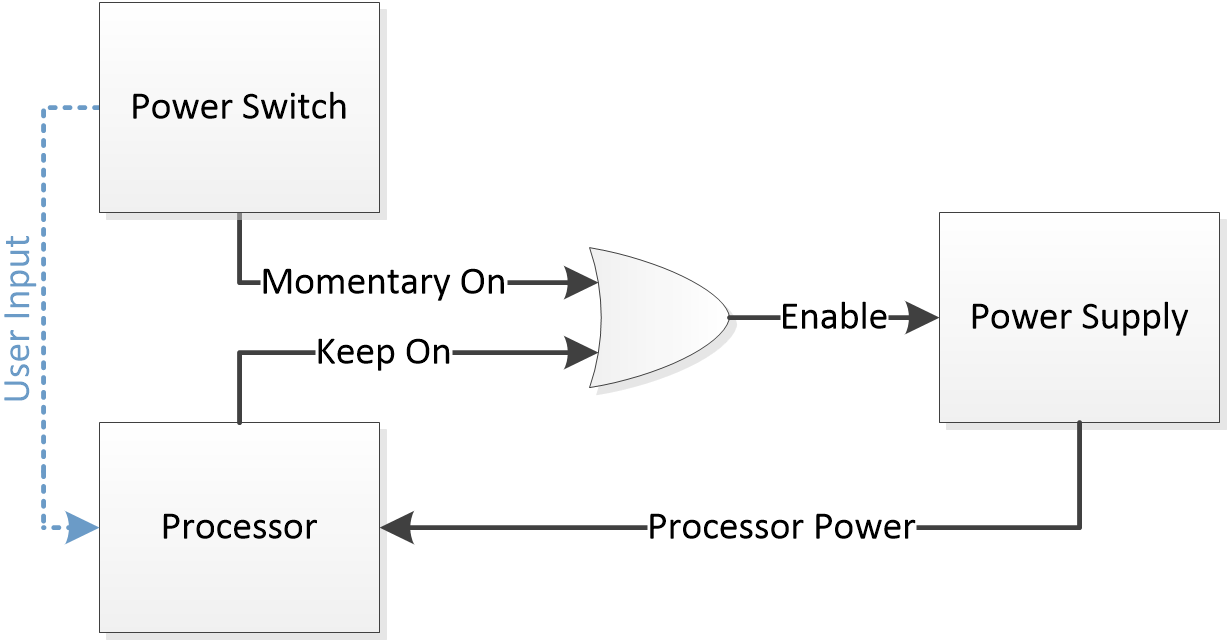
\includegraphics[width=\textwidth]{images/BlockDiagram_OnOff.png}
\caption{Simplified power on/off circuit.}
\label{fig:BlockDiagram_OnOff}
\end{figure}

The fact that the microcontroller can wait as long as it wants before turning 
itself off means that it can finish any pending IO without interruption, thus
avoiding data corruption. The “flicker” problem is also solved because the device 
can not turn on without the user pressing the button first. The isolation 
between power source and load when powered off means that standby power 
consumption should be extremely low. This implementation is slightly more 
complex and costly than the others because it uses some additional hardware 
components and relies on both hardware and software to work together, but it 
was decided that the benefits greatly outweigh the costs.

The implementation of the processor section of the schematic followed what was 
outlined in the proposal very closely. As described in 
the proposal, the design includes support for an SD card, USB communication, 
and Bluetooth communication to get data in and out of the device. All 
communication internal to the device between the microcontroller and other 
components is achieved with a combination of analog signals, GPIO pins, 
interrupt signals, I2C, and SPI. Figure \ref{fig:BlockDiagram_Processor} below 
is a block diagram showing how everything connects together.

\begin{figure}[!htb]
\centering
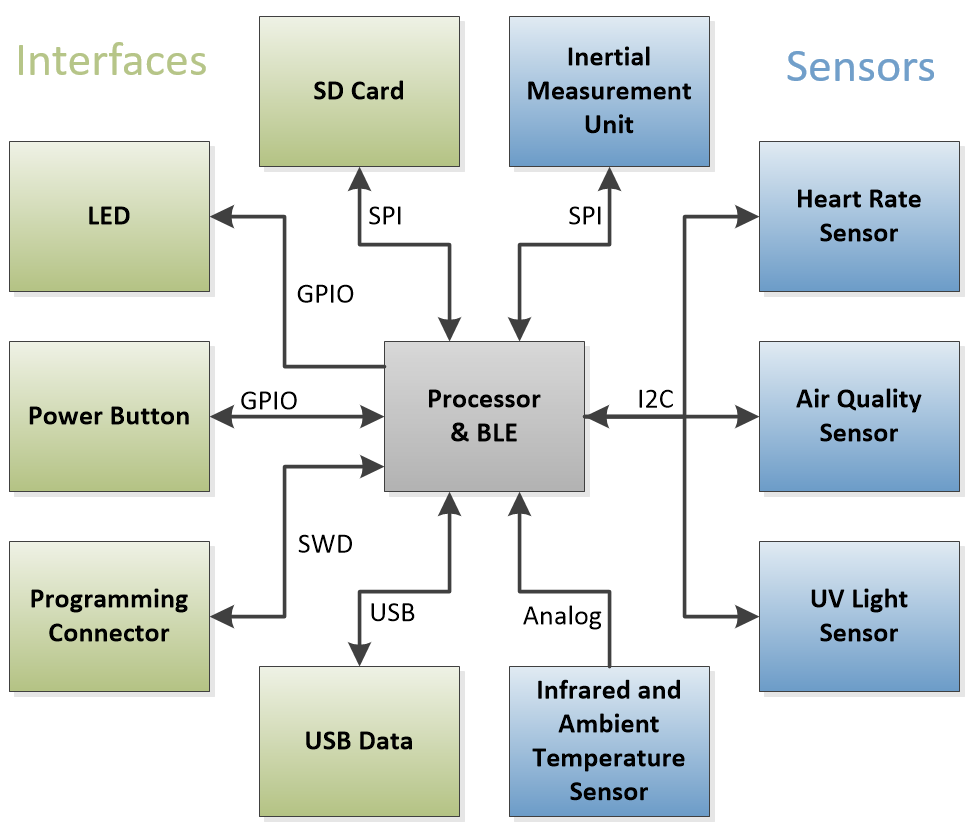
\includegraphics[width=\textwidth]{images/BlockDiagram_Processor.png}
\caption{Block diagram of processor and connected components.}
\label{fig:BlockDiagram_Processor}
\end{figure}

\subsection{PCB Layout}

The PCB design process completed with a 4-layer board measuring 35mm x 57mm as 
a result. All resistors and capacitors in the design use 0603 (Inch) size 
components because they are the smallest components available that we are
confident in being able to solder by hand. Figure \ref{fig:Board_TopBottom_Annotated}
shows an image of the circuit board as well as the locations of important 
components.

\begin{figure}[!htb]
\centering
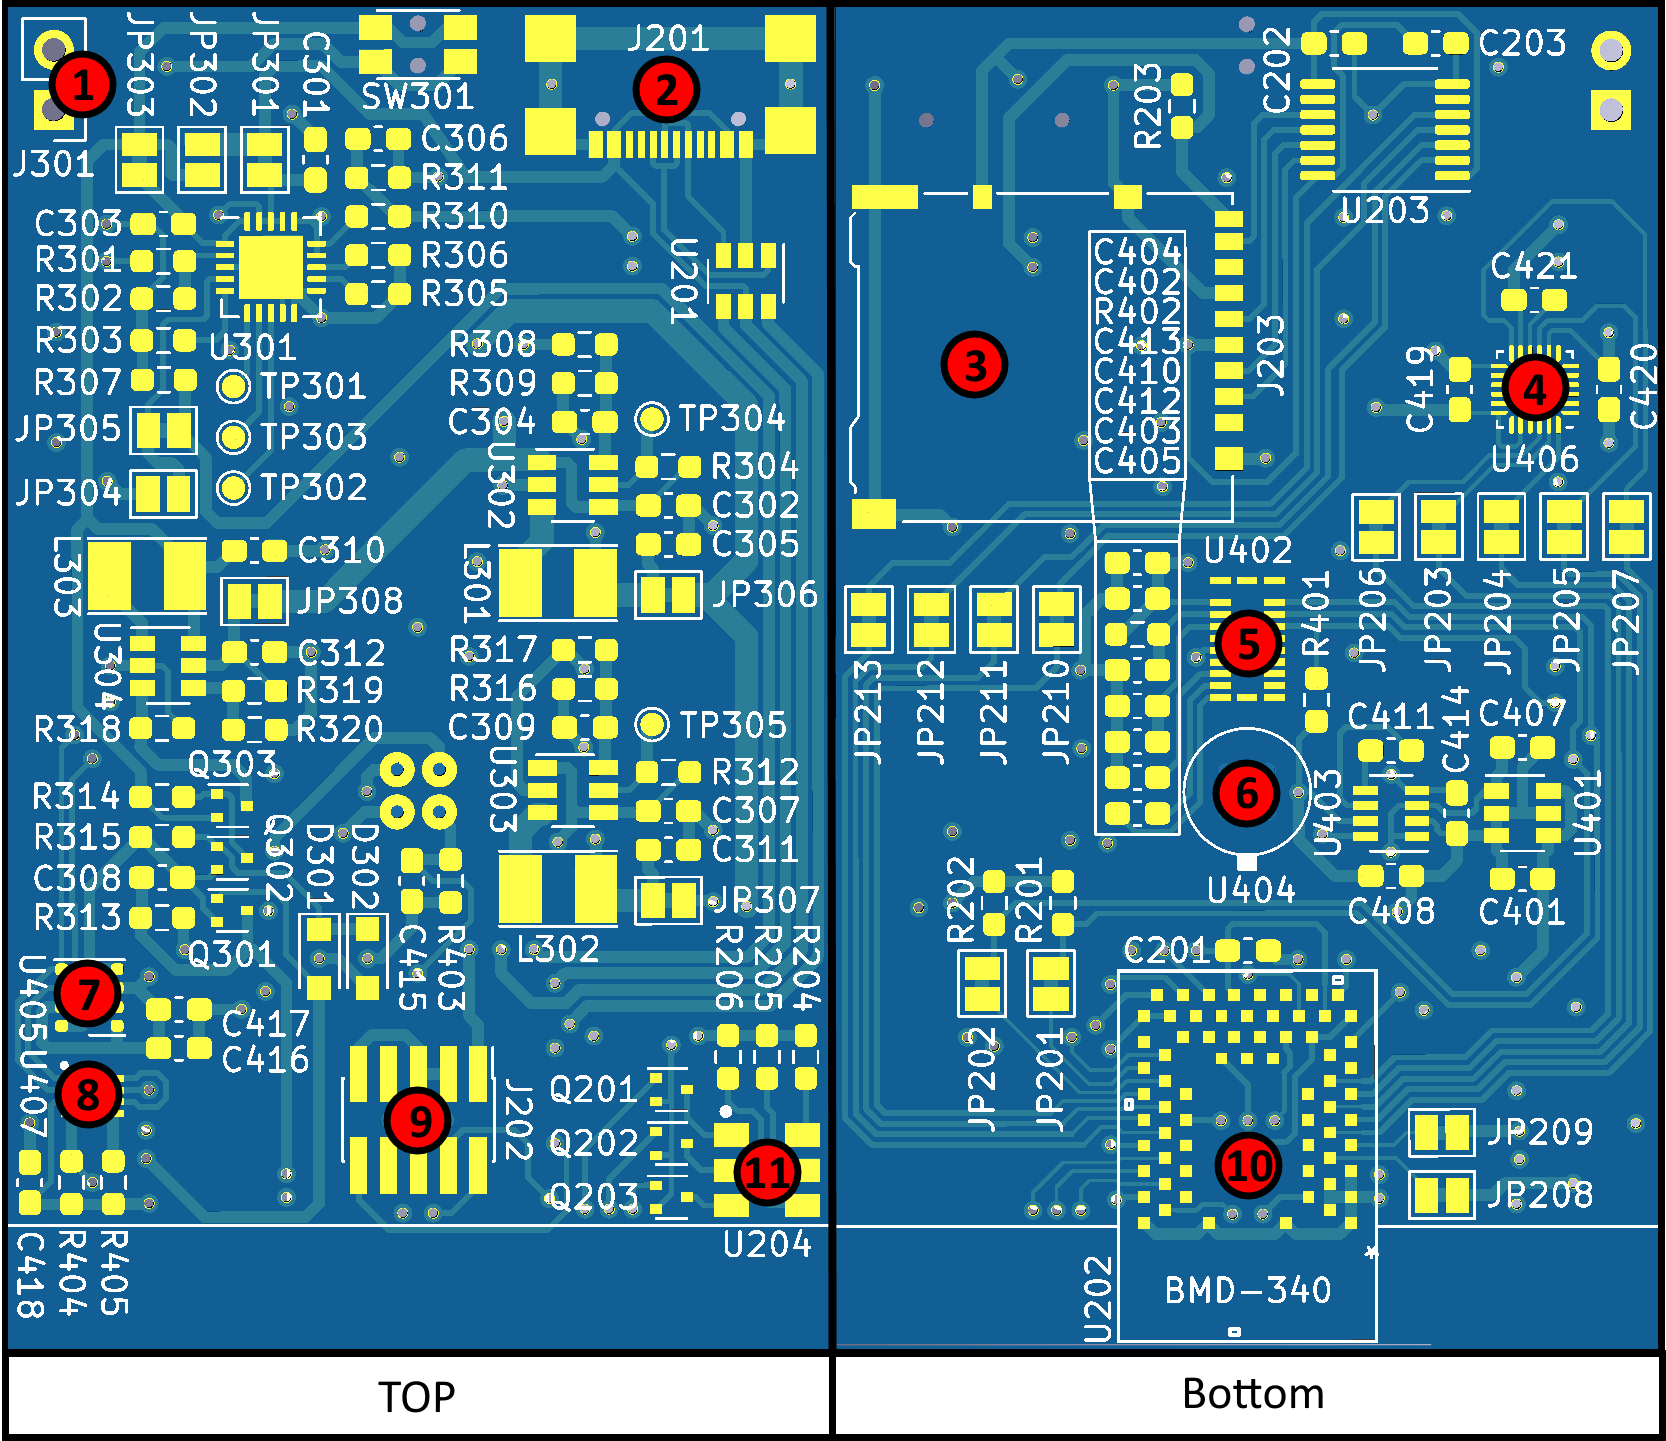
\includegraphics[width=\textwidth]{images/Board_TopBottom_Annotated.png}
\caption{CAD drawing of the completed PCB design.}
\label{fig:Board_TopBottom_Annotated}
\end{figure}

The following is a list of components indicated in Figure \ref{fig:Board_TopBottom_Annotated}: 
\begin{enumerate}
   \item LiPo battery connection
   \item USB-C port
   \item SD card slot 
   \item Inertial Measurement Unit (IMU)
   \item Heart rate sensor
   \item Infrared and ambient temperature sensor
   \item Air quality sensor
   \item UV light sensor
   \item SWD programming/debugging connector
   \item Processor module
   \item Status LED
\end{enumerate}

Placement of the components on the board was an important consideration. Many 
require proper positioning to work correctly. The USB port and SD card 
slot were placed near the edge of the board for easy access outside the 
enclosure. The heart rate sensor and infrared temperature sensor had to be 
placed on the bottom of the board so they could take measurements from the 
user’s arm. The LiPo battery will be placed on top of the board once it is 
assembled into the enclosure so that it does not block the heart rate
and temperature sensors. The status LED had to be on the top of the board so it 
could be seen by the user, but also had to be in a corner so it would not be 
covered by the battery. The air quality sensor requires access to the air outside 
the enclosure so it was placed near the edge of the board where some vents in 
the enclosure could be made. The UV light sensor had to placed on top of the 
board and also in a corner so it could receive light from outside the enclosure 
and not be blocked by the battery. The programming/debugging connector could 
have gone anywhere on the board, but the top was preferable so it could 
be accessed after the board was placed in the enclosure. The processor
module needed to have an entire edge of the board to itself, since 
recommendations from the manufacturer stated that the area around the Bluetooth 
antenna should be completely free of any metal in the PCB or elsewhere. These 
recommendations were followed closely to ensure that the Bluetooth 
communication works well in the final product. The final sensor to be placed 
was the IMU as it did not have any specific placement requirements.

\clearpage

\section{Software Implementation}
\label{sec:software}
We have split our firmware into a number of separate modules, as shown in figure
\ref{fig:fw_block_diag}. All of the drivers for microcontroller peripherals
such as serial interfaces and the ADC are provided by the nRF52 SDK, which is a
library provided by Nordic Semiconductor, the manufacturer of the nRF52840
microcontroller we are using. We are also using some higher level components
from the nRF52 SDK such as the USB CDC-ACM stack, a FAT32 filesystem driver and
Nordic's soft device S140 which is a Bluetooth LE peripheral stack.

These third party components will be used by the software we wrote ourselves
which includes the drivers for all of our sensors (IMU, optical heart rate
sensor, air quality sensor and UV light sensor) as well as the signal processing
code required to derive a heart rate from the raw data we receive from our
optical heart rate sensor. While we plan to use a third party file system
implementation we will still need to write the code that allows blocks to be
written to and read from an SD card over an SPI interface.

At the application layer we have three modules. Our data logging service is
responsible for most of the operation of our device and continually collects
and logs sensor data. The Bluetooth data transfer service facilitates accessing
the logged data over a Bluetooth interface. Our debugging interface exposes our
firmware functionality over a USB serial interface so that integration tests can
be run on the microcontroller.

\begin{figure}[!htb]
\centering
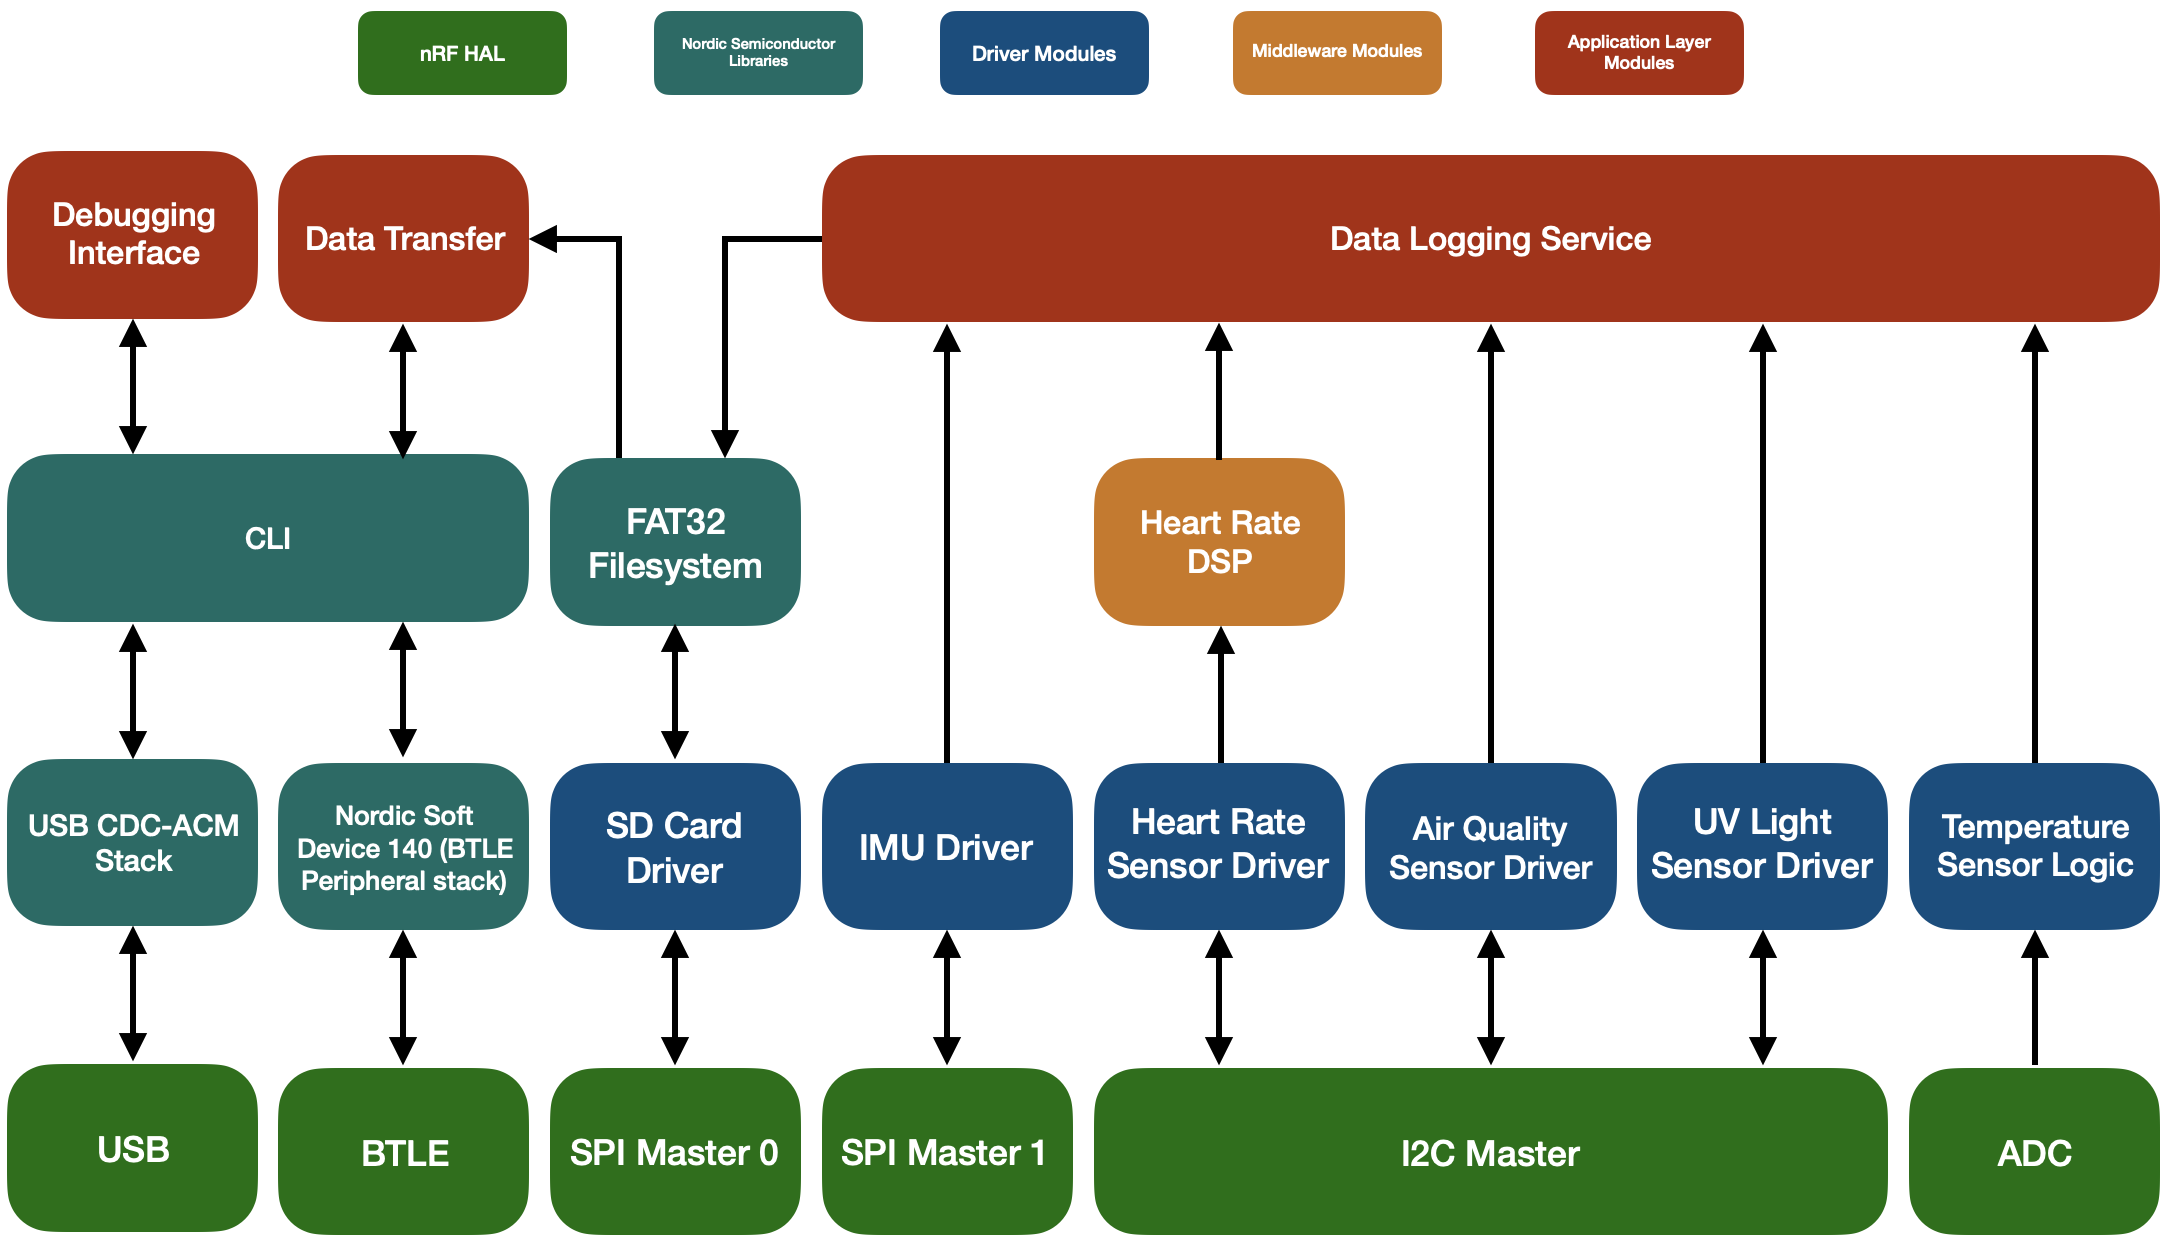
\includegraphics[width=\textwidth]{images/fw_block_diag.png}
\caption{Firmware block diagram.}
\label{fig:fw_block_diag}
\end{figure}

\subsection{Super Loop}

We chose to use a super loop architecture for our firmware because we predicted
that the approach would be sufficient for our needs and would be easier for us
to implement then making use of a realtime operating system. Our firmware
consists of an initialization section followed by an infinite main loop.

Our code is separated in to a number of software modules (as shown in figure
\ref{fig:fw_block_diag}). The software modules that we wrote have an
initialization function which is called once on system startup. Some of our
firmware module are entirely interrupt based, but many have a service function
which is run in each iteration of the main loop.

Figure \ref{fig:fw_flow} shows the flow of our firmware. We start with a number
of initialization tasks before starting to loop through the service functions
for our modules. Each service function will check if there is any work to be
done for a specific module and start and tasks that are ready to begin. After
each iteration of the main loop the wait for interrupt instruction is used to
cause the processor to enter a sleep mode until an interrupt occurs. We have a
timer configured to generate interrupts every millisecond to increment a count
which is used as a time reference throughout the firmware, because of this the
processor will sleep for at most one millisecond at a time.

\begin{figure}[!htb]
\centering
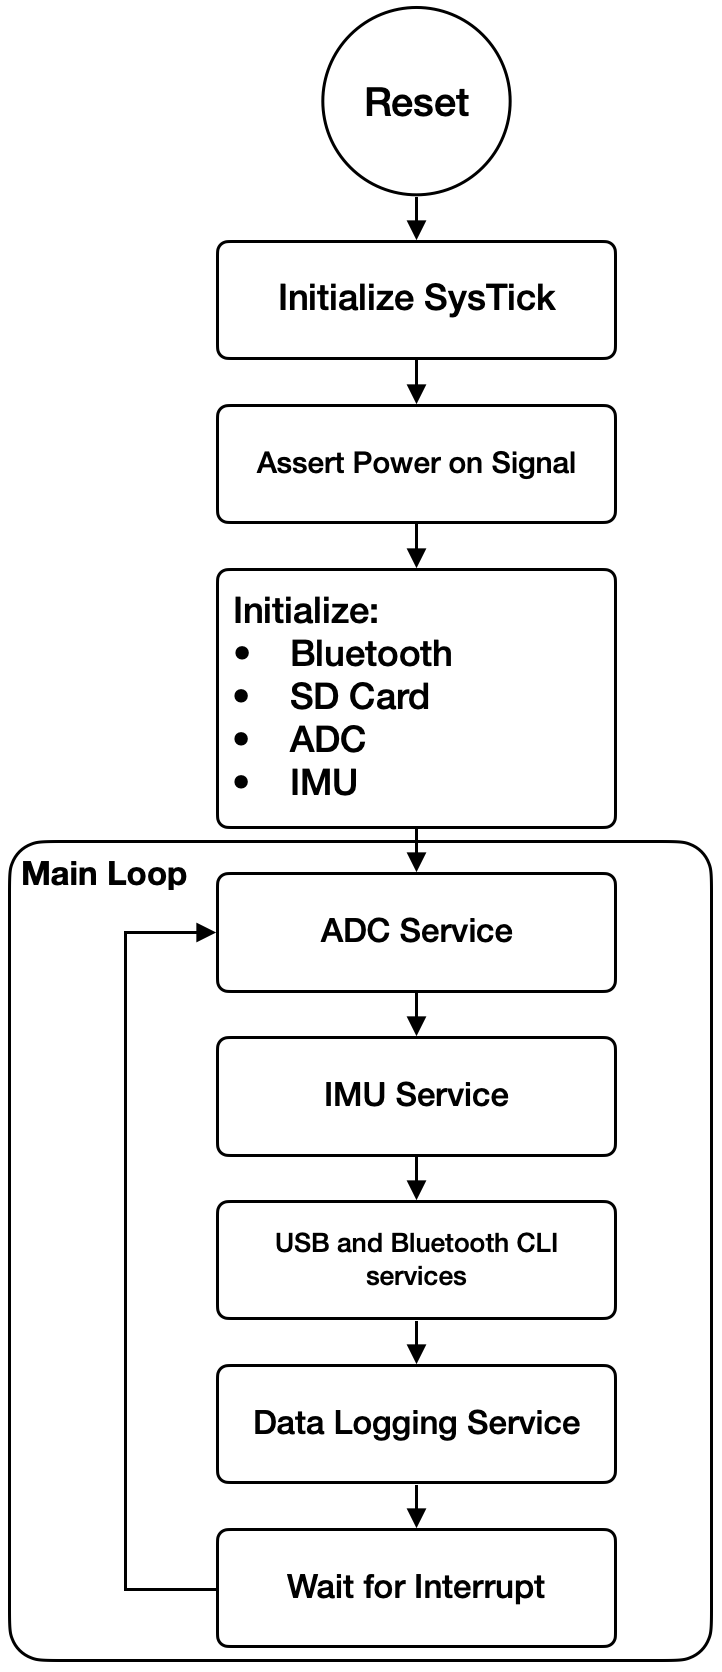
\includegraphics[width=0.4\textwidth]{images/fw_flow.png}
\caption{Firmware flow chart.}
\label{fig:fw_flow}
\end{figure}

The super loop architecture is a cooperative multitasking system. This makes it
important that the service function which are called in the main loop do not
block for long periods. If a service function was to block it would prevent the
other software modules on the system from operating correctly. In order to meet
this requirement our service functions are written as state machines. Modules
keep track of their current state and are able to determine what, if anything,
needs to be done in each iteration of the main loop based on their state.

We were not able to completely avoid blocking in the main loop because of our
use of a third party FAT filesystem implementation. The filesystem implementation
blocks while writing to the SD card. The performance implication of this are
discussed in section \ref{subsec:testing-data-logging}.

\subsection{Interrupts and Bluetooth Soft Device}

Our firmware makes use of a bluetooth stack provided by Nordic Semiconductor
know as the S140 Soft Device. This "soft device" is distributed as a binary
blob which is flashed to the microcontroller separately from the application
software. The soft device takes ownership of number of microcontroller
peripherals including the radio hardware, clock and power management peripherals,
multiple timers, non-volatile memory controller and cryptography accelerators.
The soft device schedules itself independently of the application using on of
the microcontroller's real time clocks and application software interacts with
the soft device using supervisor calls.

All interrupts are received by a piece of code called the master boot record
(MBR). The MBR then forwards them to the soft device if there is one installed
on the microcontroller. The soft device uses some interrupts for its own
purposes, interrupts which the soft device does not use are forwarded to the
application. Nordic Semiconductor specifies that this forwarding process adds
less than three microseconds of latency to peripheral interrupts which are to
handled by the application.

Figure \ref{fig:fw_int_prio} shows the interrupt priorities used in our system.
The priority levels shown in red are reserved by the soft device bluetooth
stack, those shown in blue are available for use by application software. The
soft device uses the highest interrupt priority level for its timing critical
interrupts. The second highest interrupt priority level is reserved for the
soft device's peripheral access control fault handler so that the soft device
can safely handle any faults which are caused by application interrupts. The
soft device also used priority level four for API calls and processing tasks
that are not time critical.

\begin{figure}[!htb]
\centering
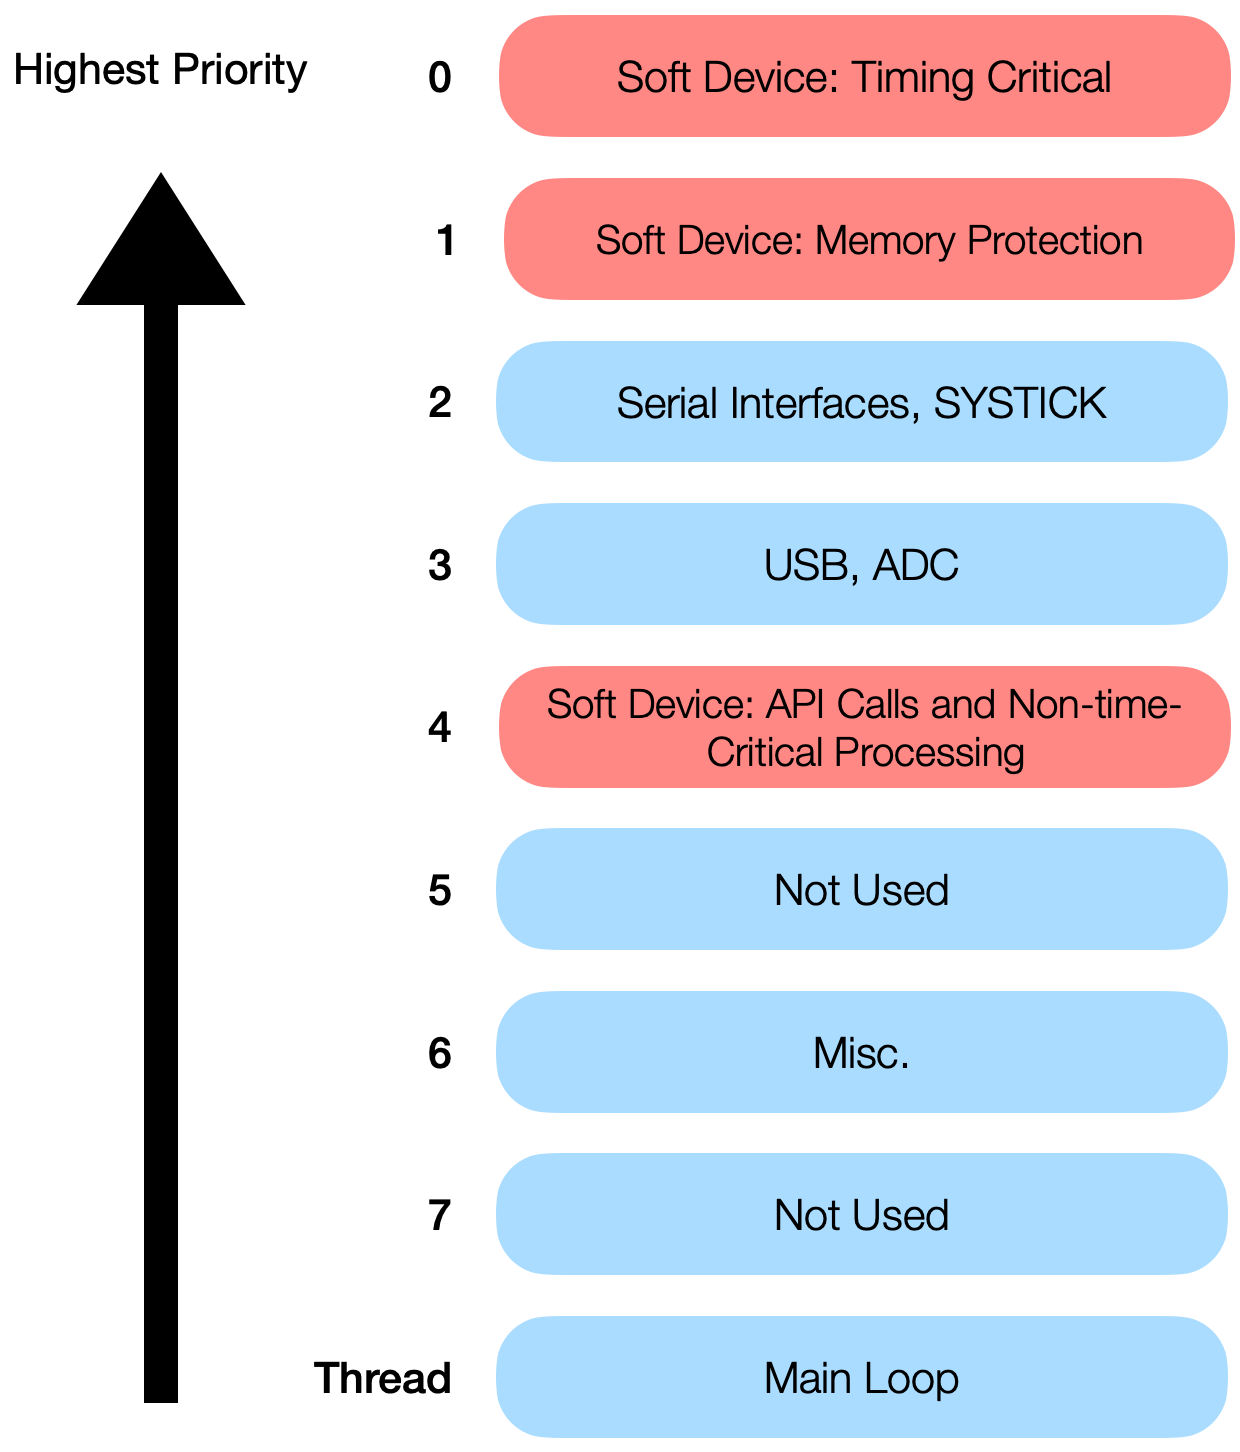
\includegraphics[width=0.5\textwidth]{images/fw_int_prio.png}
\caption{Interrupt priorities.}
\label{fig:fw_int_prio}
\end{figure}

Most of our application interrupts are configure at priority levels two and
three. Our interrupts are grouped into SysTick and and serial interface
interrupts at priority two and USB and ADC interrupts at priority three.

The priority two interrupts are those which we expect to be very short. The
SysTick interrupt is at a high priority to avoid help avoid hitter in our system
time and the serial interrupts are placed at priority two to achieve the best
possible serial interface performance.

\subsection{Data Logging}

The core of our firmware is the data logging service. Sensor drivers push data
to this software module which is buffered and then later stored to the SD card
using the FAT filesystem. The data logging module has two 512 byte buffers. The
module fills one buffer, then writes it to the SD card as it begins to fill the
other.

Figure \ref{fig:fw_data_flow} illustrates the flow of data through the data
logging service. Each sensor driver pushes data to the data logging service at a
rate selected based on the type of data that the sensor produces. Every sample
of sensor data is wrapped in a header that indicates the current system time
when the value was collected, the type of data and the length of the data and
the resulting packet is added to the data logging service buffer. Approximately
once per second the data logging buffer will be written to the SD card using the
filesystem driver.

\begin{figure}[!htb]
\centering
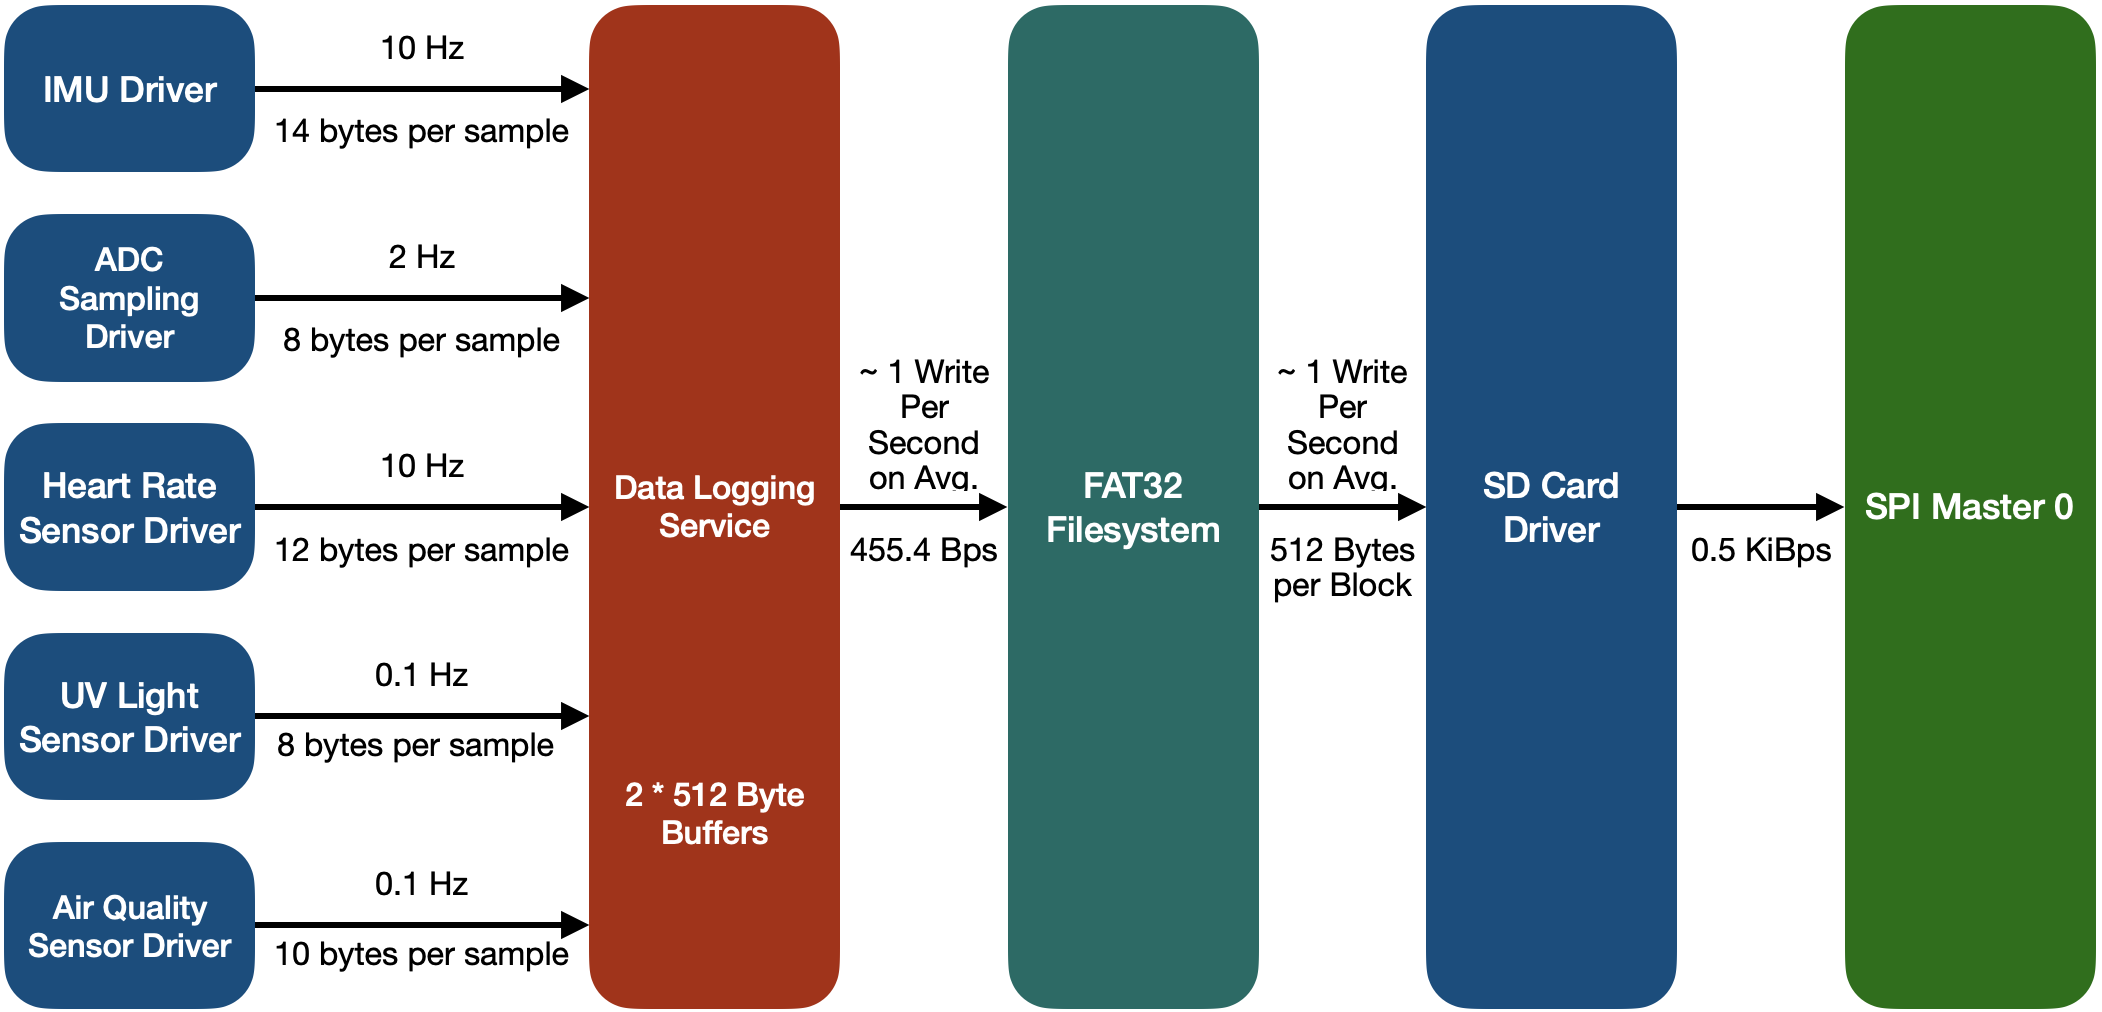
\includegraphics[width=\textwidth]{images/fw_data_flow.png}
\caption{Data flow.}
\label{fig:fw_data_flow}
\end{figure}

\subsection{Drivers}

\subsubsection{USB}

The USB serial interface software module provides a simple abstraction over the
nRF5 SDK's USB communications device class abstract communications model
(CDC-ACM) driver which allows for serial port emulation. The USB serial module
maintains circular buffers for input and output and provides a variety of
functions for reading from and writing to the buffers. The output buffer can be
written to in a blocking or non-blocking fashion. The input buffer can be read
character by character, in blocks, or by line with a selectable delimiter.

\subsubsection{Bluetooth}

The design goal for the Bluetooth driver was to have it behave like a serial
port in the same fashion that USB CDC does. Our intention in doing this was to 
simplify the design of the companion software as well as the command line 
interface present on the microcontroller. This goal was fully achieved 
on the microcontroller side of the communication link. The software interface for 
Bluetooth was made identical to USB so that they can be used interchangeably 
without additional complications. On the PC side where the companion software
runs the solution was not as elegant. We had hoped to find a way to make the
Bluetooth connection appear as a serial port so it could be used interchangeably
with the USB CDC connection, but a method to do this was not found. It likely
could be done by writing custom drivers, but this was outside the scope of the
project. Instead, a cross platform Python library was used to establish the
Bluetooth connection to the device and communicate with it as you normally
would with a Bluetooth device.

The device uses Bluetooth Low Energy, which works by advertising
available services to other nearby devices. Each service may offer a number
of characteristics that can be read only, write only, read-write, and have 
several other options such as notifying a connected device when a characteristic
value changes. The Bluetooth Low Energy specification includes descriptions of several
standard services and their characteristics, but none of these could be used to
to achieve the serial port-like behaviour needed for this project. A custom
serial port service included with the Nordic SDK was used instead. This service
has two characteristics, one named TX and one named RX. The RX characteristic is
write only and is used to send data to the device. The TX characteristic is
written to only by the device and has notifications enabled. If a connected device
wants to receive data then it must subscribe to the notifications of the TX 
characteristic. This solution worked out quite well, although it has a low 
throughput in comparison to USB. The fact that each notification packet can only 
hold approximately 20 bytes and must be acknowledged before the next one is 
sent likely contributes to the low throughput significantly. It was not expected
that Bluetooth Low Energy would be very fast however, since it is optimized for 
power consumption instead of speed. This trade-off is well suited to this project 
because it is battery powered.

\subsubsection{Heart Rate Sensor}

Our heart rate driver is based on an open source implementation written in
C++ \cite{max86150-ardino}. Since the SDK we are using falls under the nRF5
Nordic License, only software that is compatible with this license can be
integrated into the project. The open source C++ heart rate driver is under the
expat license so we are free to use it as long as the copyright notice is
maintained. Unfortunately, not all useful open source software was licensed in
a way compatible with the SDK license. In particular, it would have been ideal
to reuse an algorithm to convert raw PPG data to beats per minute, however the
available algorithm was licensed with the Lesser GNU Public
License \cite{wasp-os} which is incompatible with the SDK license.

\subsubsection{Inertial Measurement Unit}

Our driver for the ICM 20948 IMU is written from scratch. The driver is a finite
state machine that makes use of the nRF5 SDK's SPI driver. The state machine
controls the process of initializing the sensor and of periodically taking
readings, which are then handed off to the data logging service to be recorded.

A simplified state diagram for the IMU driver is shown in figure
\ref{fig:fw_imu_fsm}.

\begin{figure}[!htb]
\centering
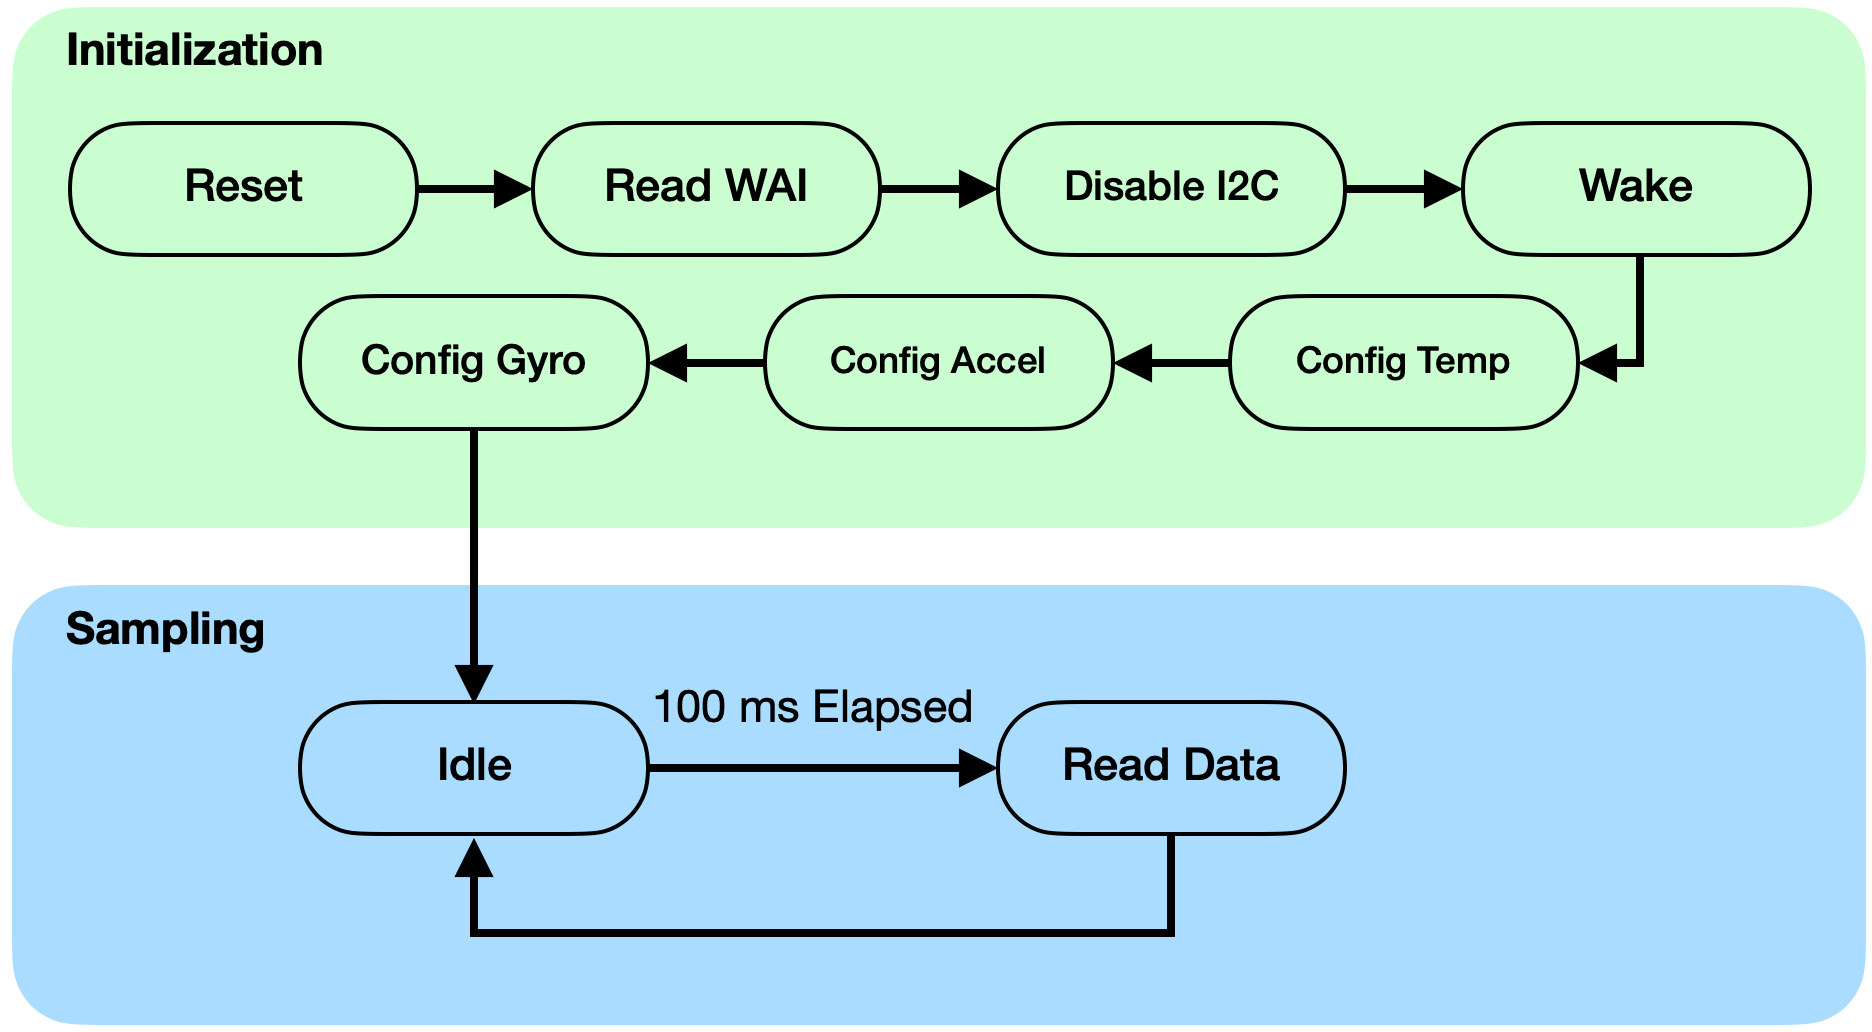
\includegraphics[width=0.8\textwidth]{images/fw_imu_fsm.png}
\caption{IMU driver state machine.}
\label{fig:fw_imu_fsm}
\end{figure}

\subsection{Command Line Interface}

Our firmware provides a command line interface (CLI) which is available via the
USB or bluetooth serial interfaces. This command line interface is used for
debugging, testing and for interaction with the companion app. Our CLI
abstraction provides an identical interface over USB or bluetooth.

The CLI provides a number of commands which are intended for human interaction
including commands for printing out sensor data, accessing profiling information,
writing test messages to the SD card and reading directories and files from the
SD card.

The CLI also has a number of commands which are intended to interact with our
companion software. These functions allow the companion software to read files
from the SD card. The files are written out over the serial interface in
hexadecimal format.

\subsection{Companion App}

The companion app is a desktop application written in python to connect to the device, extract the log data and convert it into a plain text format convenient for further analysis.

Since during development there were a number of things that were likely to change or unknown, the companion software was designed to be highly modular so that each part was isolated for sake of testing and updating.  The flow of data is described by \ref{fig:companion_app}

\begin{figure}[!htb]
    \centering
    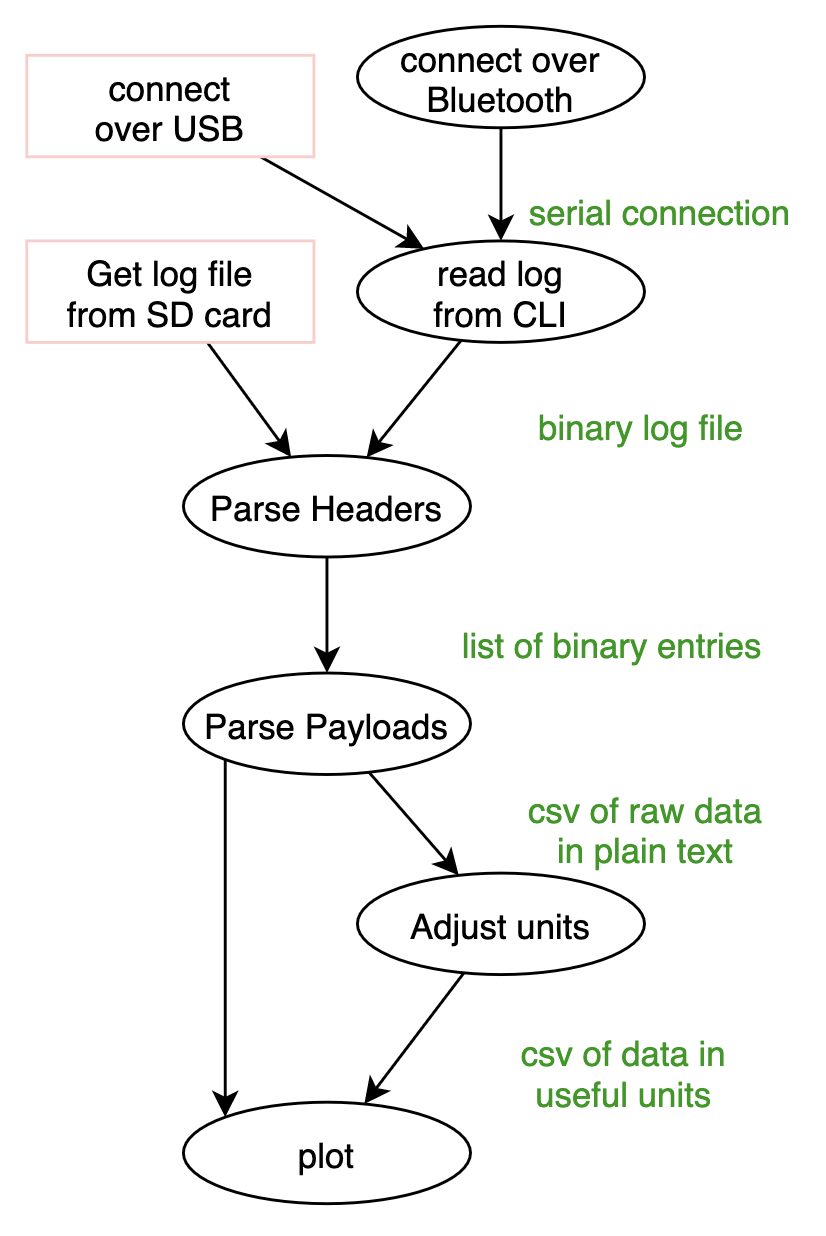
\includegraphics[width=0.6\textwidth]{images/companion_app_flow.png}
    \caption{Companion app flow diagram}
    \label{fig:companion_app}
\end{figure}
    

\subsubsection{Extracting log file}

When the device is connected over USB the companion software can be run to open a serial connection with the device, otherwise the companion software will scan for the device over bluetooth and attempt to pair and connect.  Once a bluetooth connection is established a wrapper is created to emulate the same behaviour as a serial connection so that the CLI communication module can use both connections interchangeably.

The interaction with the CLI consists of sending a time alignment command and using 'hcat' command to read the offset file and log file.  

Since the device does not have time keeping all log entries are recorded with internal timestamps only, the time alignment command creates a log entry matching an internal timestamp with a unix timestamp generated by the companion app.  

The log file consists of binary data blobs with variable length so identifying the boundaries of entries from the middle of the file is impossible without additional context, for this reason a separate file is kept with a list of offsets corresponding to each reset so an option can enable only recording data from a given reset index.

\subsubsection{Parsing log file}

Once the log file is obtained either by extracting it through the CLI interface or by extracting it from the SD card directly, it is converted from a binary format into plain text CSV files for each type of entry.

The module which parses the headers will read the length of each entry's payload and ensure the correct length of bytes is being read.  Particularly if an entry is only partially written when the device loses power a reset index specified by the separate file will indicate this and the partial entry can be discarded without corrupting all subsequent data.

The module which parses the payloads relies on introspection and struct definitions for each entry type.  The order and types of the fields are used to extract data from the log file while the name of the struct defines the name of the csv file created and the variable names in the struct are used to generate a header for the csv.  This way adding a new sensor requires only adding a struct and no additional parsing code is needed.

Unit adjustment was accounted for in the original plan however since all log entries are adjusted on the device to be fixed power of 10 of a useful unit (for example accelerometer data is $10^{-4} g$ where $g$ is a standard gravity unit) the companion app doesn't do additional adjustments. 

Some additional code is used to create a graph of a selected csv file for demonstration purposes, this also can produce live updating graphs

% TODO: talk more about live updating stuff?
% what else did I miss?

\clearpage

\section{Encolsure}
\label{sec:enclosure}

The enclosure was difficult to construct for multiple reasons.  In order to
minimize the size of the PCB, we decided to forgo traditional mounting holes.
Additionally, we avoided using adhesive to mount the PCB in order to maintain
easy access for debugging and repair purposes.  This means the enclosure needed
tight tolerances around the PCB to prevent horizontal and vertical movement.
Additionally, the sensors mounted on the bottom of the PCB need to be a precise
distance away from the users wrist.  This means the thickness of the bottom of
the enclosure needed to be accurately tuned.

To add difficulty to the situation, the enclosure was manufactured by a (rather
cheap) desktop FDM 3D printer.  These printers are known for over extruding
plastic which causes the produced part to be slightly larger in the X and Y
dimensions.  As over extruding is preferable to under extruding (which weakens
the structural integrity of the part), it is common to simply model the part
slightly smaller to compensate.

FDM printers also tend to warp parts if the plastic cools too quickly, but that
can be countered by simply putting the printer in a warm room or giving the
printer a cozy blanket (although that is a fire hazard).

However, FDM 3D printing is exceptionally fast.  They make it possible to
iterate and print a 3D model of this size multiple times per day.  This rapid
iteration has enabled us to create parts that meet the above requirements.

The need for rapid iteration has led to the creation of many parametric 3D
modeling programs.  The idea is to define variables (like the the thickness of
the bottom of the model) that can easily be changed.  The problem with many of
these modeling programs is that they simply save a series of steps the user has
entered with the GUI so they can later replay this with different values.  This
replay of events is very error prone and usually requires a lot of human
intervention.  This is because the interface makes it difficult to specify
geometry that is valid for a wide parameter range.

For this reason, OpenSCAD was used.  OpenSCAD defines 3D models in its
scripting language which is executed to produce 3D printable files.  Since
every usage of a parameter is written out explicitly, it is easy to determine
all the valid values for the parameters.

In the end, 7 iterations where needed to achieve the final enclosure. The 3D
render of the result can bee seen in Figure \ref{fig:enclosure} and the final
fabricated enclosure can be seen in Figure \ref{fig:enclosure-fab}.  Although
the board is held in place solely using friction, it is secure enough to stay in
place even during a rigorous jog while wearing the device.

\begin{figure}[!htb]
\centering
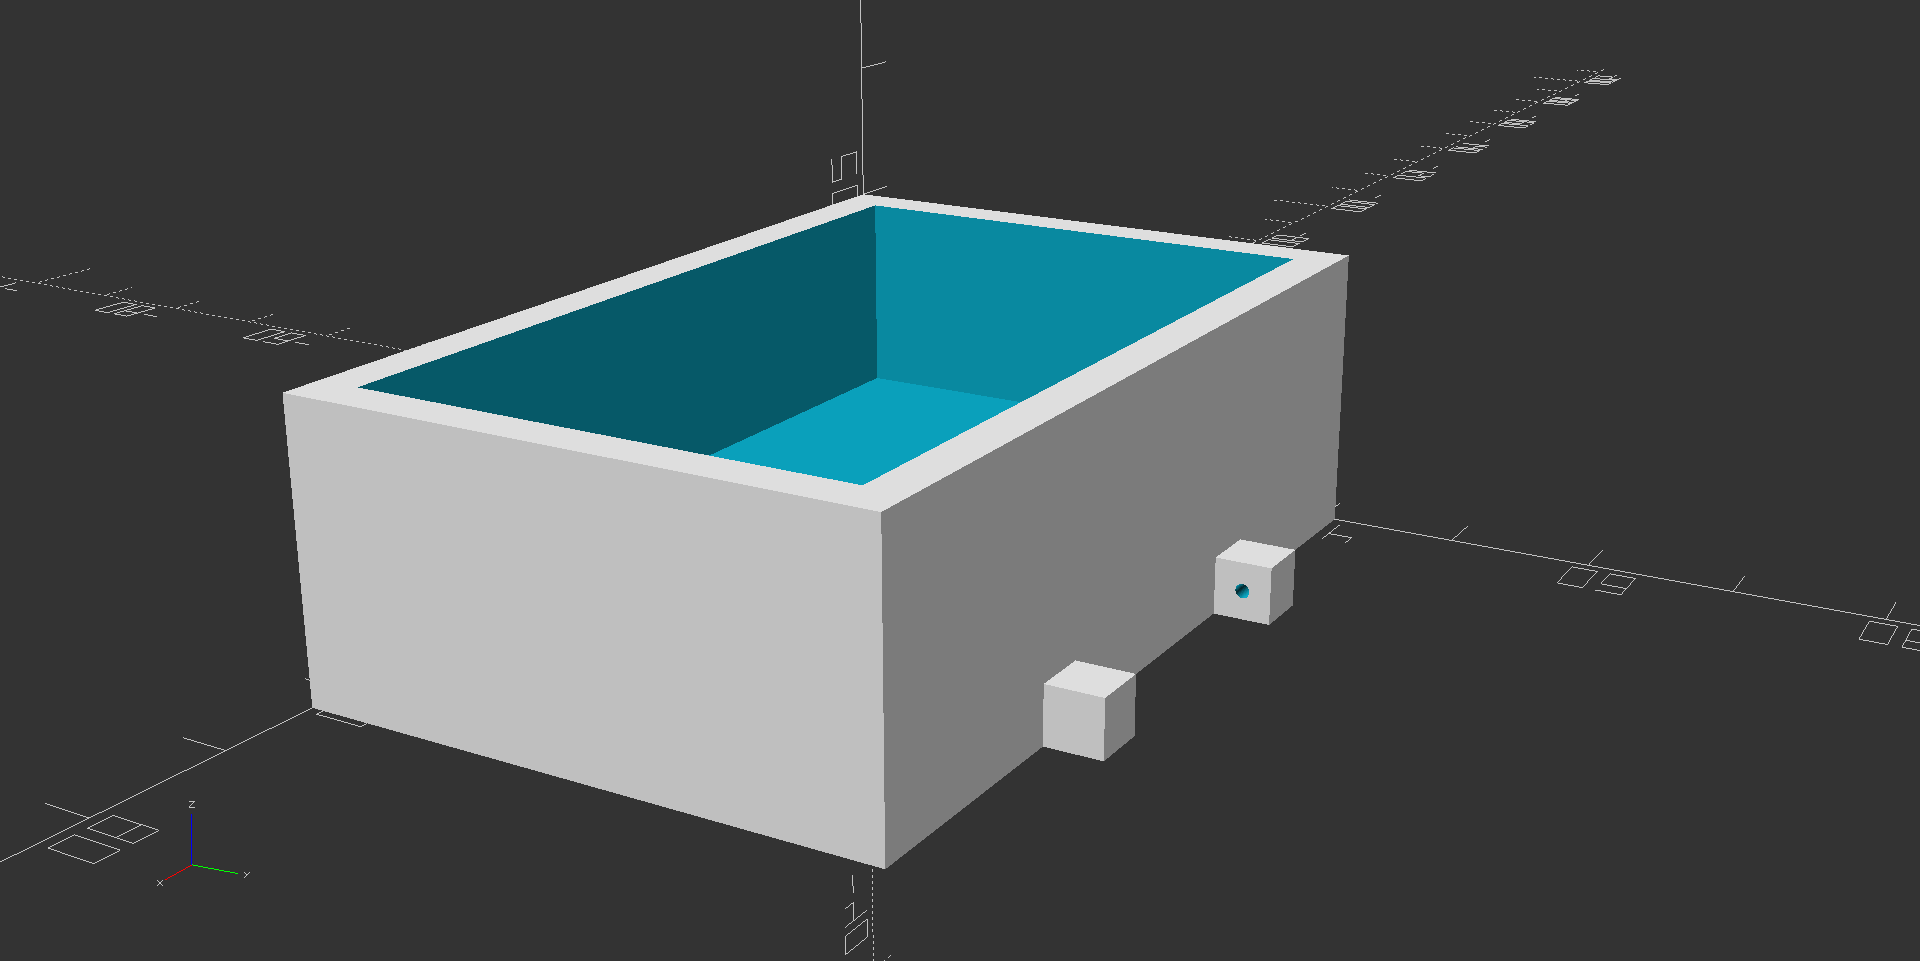
\includegraphics[width=\textwidth,height=\textheight,keepaspectratio]{images/enclosure.png}
\caption{Enclosure Render}
\label{fig:enclosure}
\end{figure}

\begin{figure}[!htb]
\centering
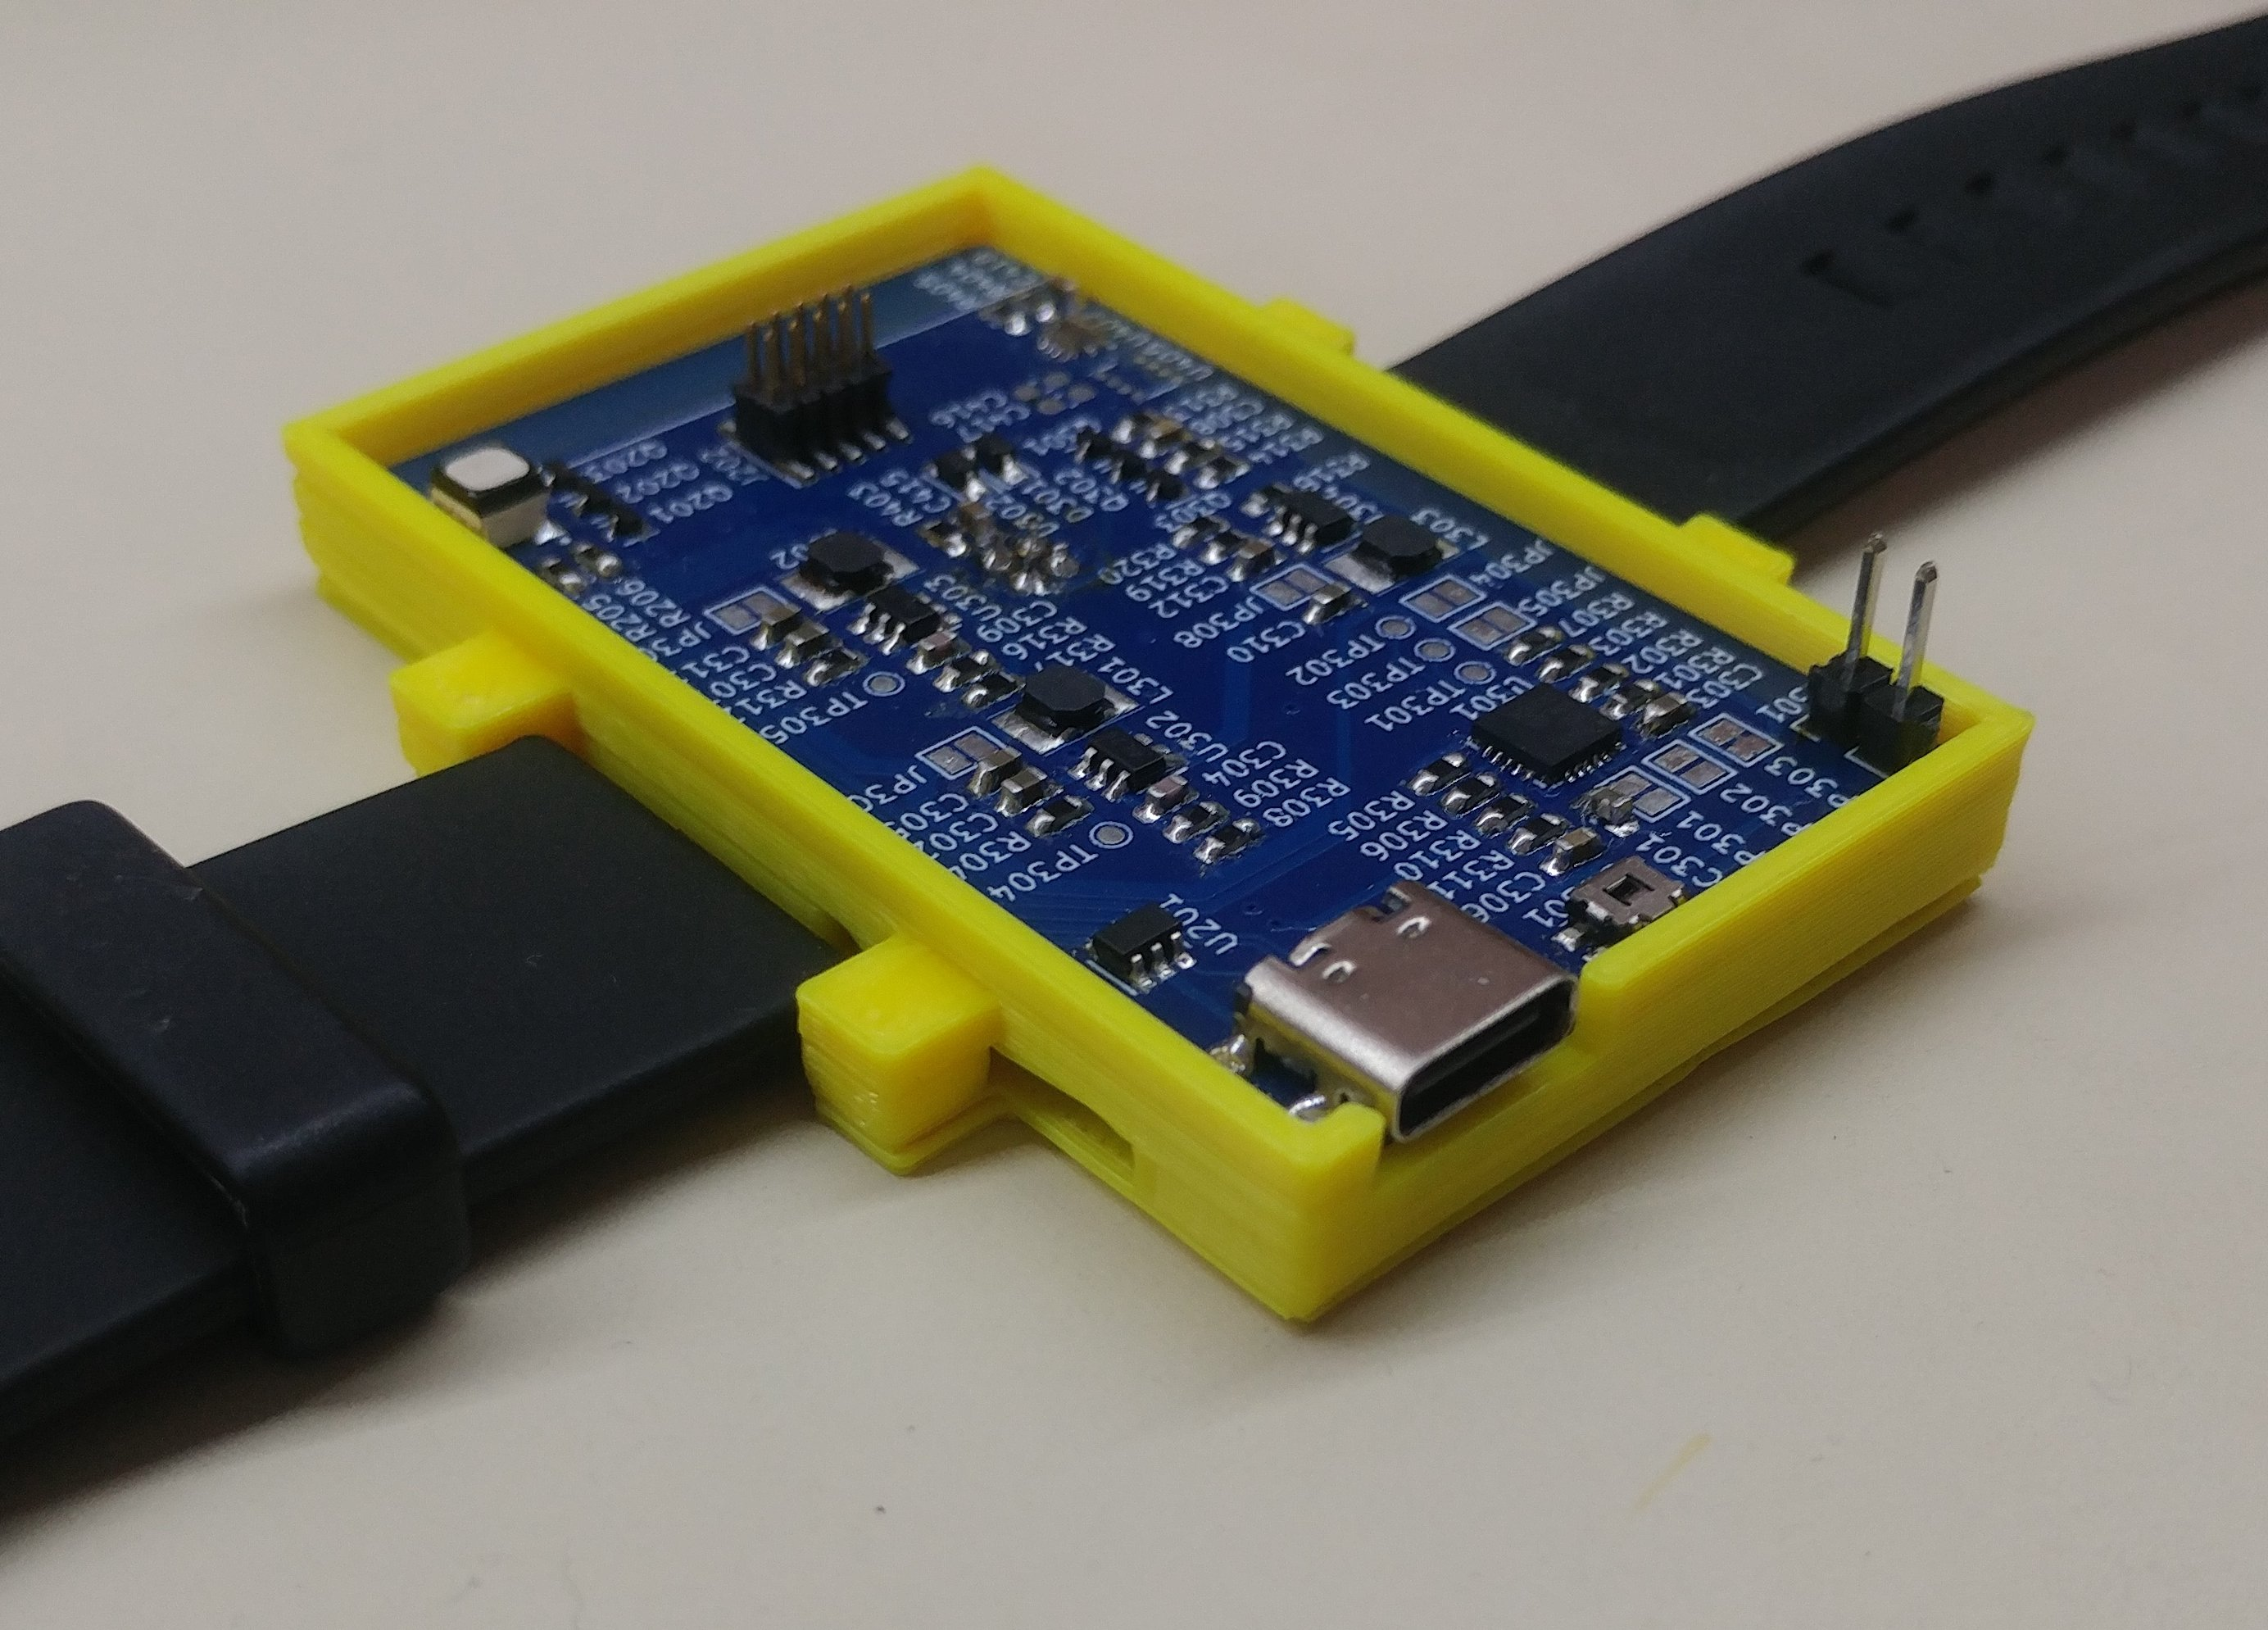
\includegraphics[width=\textwidth,height=\textheight,keepaspectratio]{images/biosense.jpg}
\caption{Fabricated Enclosure with watch straps and a board installed}
\label{fig:enclosure-fab}
\end{figure}

\clearpage

\section{Testing}
\label{sec:testing}
\subsection{Integration Testing}

\subsection{Performance Measurements}

We made a number of timing measurements for various properties of our firmware
in order to get an understanding of whether our system is able to consistently
meet its timing requirements.

Measurements where taken using a hardware timer configured to run at 8 MHz. Code
to start the timer and code to stop the timer and store the current count was
added in places of interest. For each of the measured quantities 4096 samples
were recorded.

Table \ref{table:timing-results} shows the results of our timing measurements.
For each result the mean value of all recorded samples is given as well as the
standard deviation, and maximum recorded value. For many of the recorded values
almost all of the samples were within a very small range with only a handful
of outliers, because of this a 98th percentile of deviation value is given for
each measured quantity which gives the offset from the mean in which 98\% of the
samples fall.

Later in this section some of the more illuminating measurements are described
in detail.

\begin{longtable}{>{\centering\arraybackslash}m{3.1cm}|
                >{\centering\arraybackslash}m{2.2cm}|
                >{\centering\arraybackslash}m{3.5cm}|
                >{\centering\arraybackslash}m{1.8cm}|
                >{\centering\arraybackslash}m{2.2cm}}
\toprule
Test & Mean Time & 98th Percentile of Deviation & Standard Deviation &
Maximum \\
\midrule
Time between system ticks (millis)  & 998.868 microseconds & 98\% of results
within 250 nanoseconds of the mean & 1.185e-5 & 1.077 milliseconds \\
Time spent executing body of main loop & 5.625 microseconds & 98\% of results
within 16 microseconds of the mean & 6.327e-4 & 35.071 milliseconds \\
Time spend sleeping per iteration of main loop & 931.475 microseconds & 98\% of
results are within 872 microseconds of the mean & 2.14e-4 & 994.624 microseconds
\\
Time to perform a filesystem write operation & 16.722 milliseconds & 98\% of
results are within 31.484 microseconds of the mean & 1.362e-4 & 270.318
milliseconds \\
Time between data-logging write operations & 1.196 seconds & 98\% of results are
within 32 milliseconds of the mean & 9.156e-3 & 1.378 seconds \\
Time to perform an ADC sweep (tigger to data logging call) & 154.842
microseconds & 98\% of results are within 9 microseconds of the mean & 3.359e-4
& 14 milliseconds \\
Time between ADC interrupt and handling of ADC results in main loop & 17.435
microseconds & 98\% of results are within 12.934 microseconds of the mean &
4.171e-4 & 15.854 milliseconds \\
Time to retrieve IMU sample & 42.009 microseconds & 98\% of results are within
1.249 microseconds of the mean & 2.801e-5 & 1 millisecond \\
Time between IMU samples & 101.059 milliseconds & 98\% of results are within
60.184 microseconds of the mean & 3.005e-3 & 288.711 milliseconds \\
\bottomrule

\caption{Timing Results}
\label{table:timing-results}
\end{longtable}

\subsubsection{System Tick}

The timing results show that our system tick, which is use to maintain a count
of milliseconds ('millis'), is reasonably accurate and precise.

While the average period between SysTick interrupts is slightly less then the 1
millisecond target, the count is very precise. All of the measured samples were
within 750 microseconds of the mean value and 99\% of them where within 375
nanoseconds of the mean which indicates that there is very little jitter in our
millis value.

It is also important to note that for those samples which fell further from the
mean we generally see a delayed interrupt which is immediately followed by a
shorter interrupt period, so over time the average millisecond period remains
accurate even when there is some jitter. This happens because the SysTick timer
is configured in free running mode where it is automatically cleared after each
period and continues counting without needing to be restarted in the SysTick
interrupt handler.

\subsubsection{Data-logging}

Writes to the SD card are the longest blocking operation that happens in the
main loop. On average, a write operation takes about 16.7 milliseconds, but this
is far from the whole picture.

Figure \ref{fig:write-op-hist} is a histogram showing the distribution of write
operation lengths. To make the histogram legible the data has been trimmed to
remove outliers. Only samples within the 98th percentile of deviation where
kept, leaving 4014 samples in the dataset.


\begin{figure}[!htb]
\centering

\begin{gnuplot}[terminal=pdf,terminaloptions=color]
set xlabel "Length of write operation (s)"
set ylabel "Number of occurrences"

Min = 0.00709125 # where binning starts
Max = 0.037765875 # where binning ends
n = 100 # the number of bins

width = (Max-Min)/n
bin(x) = width*(floor((x-Min)/width)+0.5) + Min

unset key
set style fill solid 0.5
set xrange [Min:Max]

%plot 'data/data_log_write_trimmed' using (bin($2)):(1.0) smooth freq with boxes
\end{gnuplot}

\caption{Distribution of Filesystem Write Operation Lengths}
\label{fig:write-op-hist}
\end{figure}

The majority of filesystem write operations take about 12.7 milliseconds, but
the distribution is multimodal and there are also a number of write operations
that take between 25 and 30 milliseconds and around 35 milliseconds. The large
number of writes that take around 12.7 milliseconds are single block writes, the
other groups of write times are 2 and 3 block write operations. This timing data
shows that most of the write operations to the SD card only need to update a
single block, but that occasionally it is necessary to update 2 or 3 blocks at
once.

\subsubsection{Main Loop}

The loop body is made up of a number of service functions which implement the
various software modules that make up the system. Ideally the main loop would
run frequently in order to provide a responsive system. This cooperative
multitasking scheme relies on each of the modules not to block for long periods
in the main loop.

For the most part the loop is very short. The vast majority of loop iterations
measured (more than 90\%) took about 5.5 microseconds. These would be loop
iterations where none of the service functions had any work to do.

Similarly, for about 90\% of loop iterations the processor spends approximately
1 millisecond sleeping. This indicates that interrupt source which wakes the
processor most frequently is the SysTick timer that is used to generate
interrupts every millisecond.

The fact that so many iterations are not performing any work is a sign that the
processor is being woken more often than it needs to be. It would likely we
worth investigating alternative ways of generating our system time value other
than with regular SysTick interrupts such as using a hardware RTC in order to
reduce how often the processor is woken.

\subsubsection{Sensor Sampling}

ADC sweeps were generally quite quick. In over 99\% of measurements the time
from when the sweep was triggered to when the results where processed was only
about 155 microseconds. The time from ADC interrupt to ADC results processing
in the main loop was less than 30 microseconds in 99\% of measurements.

There were however some outliers where ADC sweeps took significantly longer.
The longest delay between ADC interrupt and the results being processed in the
main loop was about 15.8 milliseconds. This time happens to correspond with the
delay for a single block write to the SD card and it is likely that in these
outlier cases the ADC interrupt occurred while a block write was in progress.
This implies that we could see delays of up to around 38 milliseconds in
processing ADC data, but this is not a large concern because our ADC sampling
rate is quite low.

For the IMU, the time required to read a sample from the IMU was measured. This
non-blocking operation is spread out across several iterations of the main loop.
The operation started, then later calls to the IMU service function check
whether it has completed.

In all but a handful of samples it took about 42 microseconds to read a sample
from the IMU. In the remaining samples it took slightly more than a millisecond.
These longer sample occur when the interrupt at the end of the SPI transaction
occurs while the CPU is running code in the main loop after the IMU service
function has been called. In these cases the processor will sleep again before
starting at the top of the main loop and reaching the IMU service function.

These slightly delayed IMU read operations are not a large concern to us, the
IMU sample rate is low enough that a millisecond delay will not cause us to
miss a sample and since the IMU read operation is non-blocking it does not delay
anything else happening in the main loop.

What is more concerning is the possibility of an IMU sample being delayed by
coinciding with an SD card write operation. While we did not see this in our
testing, it remains a theoretical possibility and could cause IMU samples to be
significantly delayed. It would likely be worth investigating ways to make the
SD card write operations non-blocking so that they do not interfere with other
services in the main loop.

\subsection{Power Measurements}

\subsection{Companion App Testing}





\subsubsection{Companion App Tests}

Most erroneous cases handled by the companion app are not fatal errors but warnings about skipped data. One example is that if an entry has an unrecognized type such as adding a new sensor then it is skipped and all other recognized entries are still parsed.

One notable case is that if an entry specifies it has a length of 28 bytes then
writes 10 bytes and loses power, upon reset the reset offsets file is updated with 
the length of the file and a reset command is written after the 10 bytes.  
In this case it is desirable to use the offset information in offsets to 
identify that the previous entry was not written in its entirety and discard it without allowing it to corrupt all subsequent entries.  Almost all tests for the companion app test scenarios like this where it is asserted that no fatal error was raised, the expected warning messages were given and all valid data is output as expected. As such there are no test cases to test "totally valid" data.

One case which correspond to fatal errors is when the offset specified by offsets file does not correspond to a reset command, in this case there is nothing reasonable the companion app can do to try to identify entry boundaries from the file so it gives up.  A second case which causes a fatal error is when the CLI returns the string "Failed to open file" when reading the file, as there is nothing that can be done if the SD card is corrupted and the file cannot be read, these are the only 2 fatal error cases that are tested for.

The CLI interaction is tested by creating a mock serial interface which follows the same protocols as the bluetooth or usb serial connection.  The bluetooth connection or USB serial connection are hard to write automated tests for so they are not covered by the test suite.

%We didn't do this stuff yet 
\iffalse

We plan to write automated or semi-automated tests for each component of our
project. Most of these tests will take the form of unit tests, test harnesses
that emulate adjacent modules or small test applications that exercise a single
module.

\subsubsection{Unit Tests}

We plan to build a simple unit testing framework that allows us to write unit
tests that can be compiled and run on a host system. These tests will target
individual functions and will aim to validate that they are correct.

It is unlikely that we will be able to achieve full test coverage due to time
constraints. We will therefore focus on unit testing areas of the code that
are difficult to write test harnesses for, such as sensor drivers and the SD
card driver.

\subsubsection{Sensor Driver Testing}

In addition to unit tests, we will test the sensor drivers with semi-automated
test applications that run on the microcontroller. These tests will provide
feedback over the USB-CDC interface and will interact with the actual sensor
hardware.  Our sensor tests will aim to exercise all of the functionality of the
sensors that our application code makes use of.

These tests will be in the form of small console applications that will take
a series of sensor readings and display them. These readings will be manually
verified, since automatic verification of output that is based on real world
inputs is difficult. Due to the difficulty in writing automated tests for the
sensor drivers, these drivers will be an area of focus for unit testing.

\subsubsection{Bluetooth Stack Testing}

Our Bluetooth related firmware components will be developed alongside the
companion software. As they are developed together we will test them together,
using each to verify the correct operation of the other. Much of this testing
will be performed manually as we anticipate that tests that require interaction
between our device and the companion software will be more difficult to
automate.

\subsubsection{SD Card Driver Testing}

We will test the SD card driver and filesystem software using test applications
that will run directly on the microcontroller. A test application that reads
and writes blocks on the SD card and a test application that is able to read
from and write to files will be developed in order to validate the functionality
of the SD card and filesystem code. These tests will be small console
applications that a user can interact with using the the USB-CDC interface.

\subsubsection{Data Logging Code Testing}

In order to test the data logging component of the project we will create a test
framework that runs on a desktop computer which will emulate the sensor input
and the filesystem components in order to ensure that the application layer
encryption and file packing design works as intended. This will allow the data
logging code to be developed and tested independently of the filesystem and SD
card drivers to allow for more parallel development. This test framework will
create snapshots of the outputted data for a set of input conditions and ensure
that any updates to the logging code either does not change the output to ensure
nothing is broken during development, or if there is an error in these snapshots
then the snapshots will be updated.

\fi

\clearpage

\section{Challenges}
\label{sec:challenges}
Several challenges were faced during the course of this project with both the
hardware and software development. This section will describe some of the 
challenges faced, how they were overcome, and what trade-offs or compromises,
if any, had to be considered when finding a solution.

\subsection{Hardware Challenges}

\subsubsection{Power and Battery Design}

One of the major challenges that occurred with the hardware development early
on in the project was the power supply. The original plan as described in the 
proposal was to use a single rechargeable AAA nickel metal hydride (NiMH) 
battery. Designing a power supply to work with the low input voltage of 1.2V 
to 1.0V proved to be quite difficult due to a small selection of components that 
work at that voltage. The most difficult part was trying to implement a soft 
power on / off circuit as well as an automatic switchover circuit to shift the 
electrical load from the battery to USB power. The voltage drop across a diode 
for example makes the resulting signal nearly unusable to turn on a MOSFET. 
Diodes with a very low forward voltage drop and MOSFETS with very low gate 
threshold voltages are available for a higher price, but keeping cost down was 
also a very important goal. In the end a design was created, and since it was 
expected that it may present some problems, it was prototyped on a breadboard 
so that testing could be done before moving ahead with schematic capture and 
PCB design.

Testing showed that the design mostly worked, but had some flaws that were 
deemed unacceptable for this project. The first concern was that the power 
supply would not be able to supply enough current. It was capable of powering 
an nRF52840 development board with some additional resistive load, but it 
struggled to maintain a set voltage and it became apparent that it would be 
barely capable of powering the final design with several sensors. The second 
issue was with voltage regulator start up under load. The switching regulator 
was only able to start with a very small load on it, but once the output had 
reached the desired voltage more load could be placed on it without issue. When 
too much load was attached to the regulator before start up it would stay in an 
under-voltage lockout state indefinitely. This problem may or may not have 
presented itself in a real-world test with the final design, however the goal 
was to have a robust solution that was reliable and not leave things to chance 
with a potential race condition. The final problem was efficiency. With a light 
load the power supply performed in an acceptable fashion, but under heavier 
loads efficiency dropped off much more than expected. The datasheet for the 
regulator did not indicate that efficiency would change appreciably over the 
range of current being drawn for testing, but it did indicate that lower input 
voltages would cause a significant decrease in efficiency. It is believed that 
higher load caused the battery voltage to drop due to its series resistance 
which then caused the regulator to draw much more current to account for the 
higher load and decreased efficiency at the same time because of the decreased 
input voltage. Replacing the battery with a lab power supply set to constant 
voltage showed the expected efficiency under both light and heavy loads. For 
these three reasons it was decided that the original idea of using a single 
rechargeable AAA NiMH battery was not feasible. 

At this point the group had to decide between using two AAA NiMH batteries in 
series to increase the voltage, or starting over and using a LiPo battery. It 
was decided that two AAA batteries would be too large, so the switch to LiPo 
was made and the power supply was subsequently redesigned to reflect these 
changes. One of the design requirements in the proposal was to have the 
batteries removable so they could be swapped out with charged ones instead of 
waiting for the device to charge them. This will no longer be possible with 
the current design; however fast charging capability has now been added as a 
replacement.

\subsubsection{Assembly and Parts Availability}

One of the key challenges that we planned for and managed on the hardware side
of our project was the difficulty of assembling our circuit boards by hand. Due
to the sensors we wanted to use coming in packages designed for small, high
density printed circuit board designs and our desire to build a prototype that
was roughly wrist sized we ended up using a number of components that were not
particularly well suited to hand assembly.

For the most part our assembly still worked out well using a hot air reflow
technique, but we did encounter significant frustration and delay in soldering
our microcontroller module to the board. The module we used was not amenable to
the hot air reflow technique since the pads that needed to be soldered are
located below an RF shielding can. This means that it took a considerable amount
of time and heat to properly reflow the solder paste below the module and we had
inconstant results with no way of properly inspecting the module to ensure that
it had been soldered properly. In the end we simply ended up repeatedly removing
the module and then soldering it back on until we were lucky enough to have all
of the pins flow properly.

An issue that we did not foresee, but should have, was limited availability of
components. When originally designing our hardware we limited ourselves to
components that were readily available in small quantities from online
retailers and that were in stock in large quantities at the time. Between
finalizing our schematic design near the end of the fall semester and ordering
the components for our first copy of the board in the winter semester the IMU
and air quality sensors we had selected had gone out of stock at all of the
electronics retailers that we were familiar with. The IMU later became
available again, but we were never able to obtain the air quality sensor.

A few weeks later when we went to order parts for our second copy of the board
we found that even more components had become unavailable. In addition to the
air quality sensor, the microcontroller module, diodes, USB connector and UV
light sensor that we had chosen for our design were not available. We were
able to find a substitute microcontroller module, though the substitute requires
an external Bluetooth antenna and suitable replacement diodes, but we were
forced to leave the USB connector and UV light sensor unpopulated on the second
copy of our board.


\subsection{Software Challenges}

\subsubsection{Toolchain and nRF5 SDK}
\label{sec:toolchain-issues}

Our toolchain setup ended up being much more difficult than we had envisioned.
In our proposal we had only budgeted ourselves a couple days for this step,
assuming that our experience with other ARM microcontrollers would allow us to
get up and running with the nRF52840 quite quickly. In reality, this seemingly
simple task had required a significant investment of time which held up our
software progress early in the project considerably.

We are used the hardware abstraction layer provided by Nordic
Semiconductor for the nRF52840 as well as some of their libraries. While we had
a build system set up that allowed us to successfully compile and run bare metal
software without any of Nordic's nRF SDK components, actually compiling the SDK 
along with our own code proved to be significantly more challenging. We 
originally tried to adopt our custom Makefile to also compile the nRF52 SDK files 
we required, but ended up having to base our project layout off of one of the 
example projects provided with the nRF52 SDK. A surprising amount of work was 
required to get the Makefile and Segger Embedded Studio project from the example 
to work in our repository without having to place all of our code in the examples 
folder inside the nRF52 SDK's directory structure. The makefiles provided in the
nRF52 SDK are inflexible and make use of a large number of hard coded paths.

\subsubsection{USB and Bluetooth Integration}

One of the challenges faced during integration testing was a conflict between 
the USB and Bluetooth drivers. The two drivers were developed independently of
each other, and both worked on their own. When running the two drivers together
Bluetooth would function as expected but USB would fail to enumerate on the host
and therefore, not work at all. Oddly, this problem would not occur when the 
microcontroller was running in debug mode, it presented itself only in the 
normal run mode. This made the problem much more difficult to solve because
stepping though code, breakpoints, or any other debugging capabilities were not
available outside of debug mode. The alternative technique used was to turn on 
an LED when execution reached a certain point or some condition was met. 

In the end, the solution to the problem ended up being very easy to implement 
despite taking a significant amount of time to find. When Bluetooth is 
initialised, it enables what Nordic calls a Soft Device. This Soft Device runs 
the Bluetooth stack and also takes over control of some parts of the hardware 
in the process. If other components of the software need access to hardware 
controlled by the Soft Device, then they must make calls to the Soft Device to 
perform the necessary actions on their behalf. The USB driver relies on events 
from the hardware to inform it when it is attached to a host so it knows when 
to enumerate and begin communicating. These hardware events happen to be blocked 
by the Soft Device, so if the USB driver wants to receive them it must arrange 
this with the Soft Device after it has been enabled. The USB initialisation 
functions provided by the Nordic SDK will check if the Soft Device is enabled or 
not and set things up accordingly. The problem we experienced was a result of 
initialising USB first, then Bluetooth, which in turn enables the Soft Device. 
At the time USB was initialised, the Soft Device was not enabled so the SDK did 
not set up the hardware events to work with the Soft Device. Once the Soft Device 
was enabled by the Bluetooth initialisation, the hardware events would no longer 
work for USB. The result was the USB driver not knowing the device had been 
connected to a host, so it would remain idle and never make any attempt to 
enumerate or communicate with the host. While running in debug mode, there just
happened to be enough time for the hardware events to reach the USB driver after 
it was initialised but before Bluetooth was initialised. The solution to the problem
was to simply enable the Soft Device in the USB initialisation code before it
configures the hardware for USB detection. This way, when the SDK checks if the
Soft Device is enabled it will see that it is, and USB will be configured 
accordingly.

\clearpage

\section{Timeline}
\label{sec:timeline}
Our original timeline was very optimistic.  Our original timeline can be seen
in figure \ref{fig:original-project-timeline} and our actual timeline can be
seen in figure \ref{fig:final-project-timeline}.

Software development was started much later than intended. There are a few
explanations for this.  The software development environment was more
difficult to set up than expected.  Also there was a discouraging lack of
feedback since there was no hardware to test on.

The most prominent change in hardware is the elimination of a second PCB
revision. Thankfully, only having one revision did not prevent us from making a
functional product, but this eliminate was done to save time, not because we
had a flawless first PCB revision.

The enclosure was delayed due to hardware assembly and part availability
issues.  The idea behind the enclosure design was to rapidly iterate the case
with the PCB in hand.  However, assembly and part availability issues meant the
hand off of the PCB to the case designer happened much later than expected.


\ganttset{
    calendar week text={\currentweek},
    y unit title=0.5cm, y unit chart=0.5cm,
    vgrid,
    x unit = 1mm,
    time slot format=isodate,
    time slot unit=day,
    title/.append style={draw=none, fill=RoyalBlue!50!black},
    title label font=\sffamily\scriptsize\color{white},
    title label node/.append style={below=-1.6ex},
    title left shift=.05,
    title right shift=-.05,
    title height=1,
    bar height=.6,
    group right shift=0,
    group top shift=.6,
    group height=.3,
    group peaks height=.2,
    bar incomplete/.append style={fill=Maroon},
    bar label node/.style={text width=3cm,align=right,font=\scriptsize\RaggedLeft,anchor=east},
    milestone label node/.style={text width=2cm,align=right,font=\scriptsize\RaggedLeft,anchor=east},
    group label node/.style={text width=3cm,align=right,font=\textbf\scriptsize\RaggedLeft,anchor=east},
    bar/.append style={opacity=0.5}
}

\newcommand\mygantttitle {
    \gantttitlecalendar{year} \\
    \gantttitlecalendar{month} \\
    \gantttitlecalendar{week}
}

\newcommand\proposalColor{blue!70}
\newcommand\progressColor{red!70}
\newcommand\finalColor{green!70}

\newcommand\proposalBar[3]
{\ganttbar[bar/.append style={fill=\proposalColor}]{#1}{#2}{#3}}
\newcommand\progressBar[3]
{\ganttbar[bar/.append style={fill=\progressColor}]{#1}{#2}{#3}}
\newcommand\finalBar[3]
{\ganttbar[bar/.append style={fill=\finalColor}]{#1}{#2}{#3}}

\newcommand\ProposalProgressBar[5]
{\proposalBar{#1}{#2}{#3}\progressBar{}{#4}{#5}}

\newcommand\ProgressFinalBar[5]
{\progressBar{#1}{#2}{#3}\finalBar{}{#4}{#5}}

\newcommand\ProposalFinalBar[5]
{\proposalBar{#1}{#2}{#3}\finalBar{}{#4}{#5}}

\begin{figure}[!htb]
\makebox[\textwidth][r]{
\begin{ganttchart}[]{2020-11-02}{2021-03-20}
    \mygantttitle \\
% Software
    \ganttgroup{Software}{2020-11-02}{2021-02-20} \\
    \ganttbar{Setup Dev. Env.}{2020-11-02}{2020-11-07} \\
    \ganttbar{USB Debugging Interface}{2020-11-08}{2020-12-19} \\
    \ganttbar{SD Card Driver}{2020-11-08}{2021-01-02} \\
    \ganttbar{Sensor Drivers}{2020-11-08}{2021-01-09} \\
    \ganttbar{Filesystem}{2020-12-12}{2021-01-16} \\
    \ganttbar{Bluetooth Interface}{2020-12-19}{2021-01-30} \\
    \ganttbar{Data Logging}{2020-12-26}{2021-01-30} \\
    \ganttbar{Companion Software}{2021-01-02}{2021-02-20} \\

% Testing
    \ganttbar{Sensor Driver Tests}{2021-01-09}{2021-02-13} \\

% Elec
    \ganttgroup{Hardware}{2020-11-02}{2021-03-06} \\
    \ganttbar{Electrical Schematic}{2020-11-02}{2020-12-12} \\
    \ganttbar{PCB Rev. A}{2020-12-13}{2021-01-30} \\
    \ganttbar{PCB Rev. B}{2021-01-31}{2021-03-06} \\

% Mech
    \ganttgroup{Enclosure}{2020-11-02}{2021-03-08} \\
    \ganttbar{Enclosure Prototype A}{2020-11-02}{2020-12-19} \\
    \ganttbar{Enclosure Prototype B}{2021-01-23}{2021-02-03} \\
    \ganttbar{Final Enclosure}{2021-02-27}{2021-03-08} \\
\end{ganttchart}
}
\caption{Original Project Timeline}
\label{fig:original-project-timeline}
\end{figure}

\begin{figure}[!htb]
\makebox[\textwidth][r]{
\begin{ganttchart}[]{2020-11-02}{2021-03-20}
    \mygantttitle \\
% Software
    \ganttgroup{Software}{2020-11-02}{2021-03-08} \\
    \ganttbar{Setup Dev. Env.}{2020-11-02}{2020-12-24} \\
    \ganttbar{USB Debugging Interface}{2020-12-25}{2021-01-22} \\
    \ganttbar{SD Card Driver}{2021-01-15}{2021-02-01} \\
    \ganttbar{Sensor Drivers}{2021-01-15}{2021-02-12} \\
    \ganttbar{Filesystem}{2021-01-22}{2021-02-19} \\
    \ganttbar{Bluetooth Interface}{2021-01-29}{2021-02-26} \\
    \ganttbar{Data Logging}{2021-02-05}{2021-02-19} \\
    \ganttbar{Companion Software}{2021-02-12}{2021-03-08} \\

% Testing
    \ganttbar{Sensor Driver Tests}{2021-02-05}{2021-03-08} \\

% Elec
    \ganttgroup{Hardware}{2020-11-02}{2021-03-06} \\
    \ganttbar{Electrical Schematic}{2020-11-02}{2020-12-24} \\
    \ganttbar{PCB Layout}{2020-12-24}{2020-12-31} \\
    \ganttbar{PCB Assembly}{2021-01-20}{2021-02-10} \\

% Mech
    \ganttgroup{Enclosure}{2021-01-01}{2021-02-26} \\
    \ganttbar{Enclosure Prototype}{2021-01-01}{2021-01-25} \\
    \ganttbar{Final Enclosure}{2021-02-12}{2021-02-26} \\
\end{ganttchart}
}
\caption{Progress Report Timeline}
\label{fig:progress-timeline}
\end{figure}

\begin{figure}[!htb]
\makebox[\textwidth][r]{
\begin{ganttchart}[]{2020-11-02}{2021-03-20}
    \mygantttitle \\
% Software
    \ganttgroup{Software}{2020-11-02}{2021-03-08} \\
    \ProposalProgressBar{Setup Dev. Env.}{2020-11-02}{2020-11-07}{2020-11-02}{2020-12-24} \\
    \ProposalProgressBar{USB Debugging Interface}{2020-11-08}{2020-12-19}{2020-12-25}{2021-01-22} \\
    \ProposalProgressBar{SD Card Driver}{2020-11-08}{2021-01-02}{2021-01-15}{2021-02-01} \\
    \ProposalProgressBar{Sensor Drivers}{2020-11-08}{2021-01-09}{2021-01-15}{2021-02-12} \\
    \ProposalProgressBar{Filesystem}{2020-12-12}{2021-01-16}{2021-01-22}{2021-02-19} \\
    \ProposalProgressBar{Bluetooth Interface}{2020-12-19}{2021-01-30}{2021-01-29}{2021-02-26} \\
    \ProposalProgressBar{Data Logging}{2020-12-26}{2021-01-30}{2021-02-05}{2021-02-19} \\
    \ProposalProgressBar{Companion Software}{2021-01-02}{2021-02-20}{2021-02-12}{2021-03-08} \\

% Testing
    \ProposalProgressBar{Sensor Driver Tests}{2021-01-09}{2021-02-13}{2021-02-05}{2021-03-08} \\

% Elec
    \ganttgroup{Hardware}{2020-11-02}{2021-03-06} \\
    \ProposalProgressBar{Electrical Schematic}{2020-11-02}{2020-12-12}{2020-11-02}{2020-12-24} \\
    \proposalBar{PCB Rev. A}{2020-12-13}{2021-01-30} \\
    \proposalBar{PCB Rev. B}{2021-01-31}{2021-03-06} \\
    \progressBar{PCB Layout}{2020-12-24}{2020-12-31} \\
    \progressBar{PCB Assembly}{2021-01-20}{2021-02-10} \\

% Mech
    \ganttgroup{Enclosure}{2020-11-02}{2021-03-08} \\
    \ProposalProgressBar{Enclosure Prototype A}{2020-11-02}{2020-12-19}{2021-01-01}{2021-01-25} \\
    \proposalBar{Enclosure Prototype B}{2021-01-23}{2021-02-03} \\
    \ProposalProgressBar{Final Enclosure}{2021-02-27}{2021-03-08}{2021-02-12}{2021-02-26} \\
\end{ganttchart}
}
\begin{itemize}
    \item \colorbox{rgb:\proposalColor,1;white,1}{Proposal Report Timeline}
    \item \colorbox{rgb:\progressColor,1;white,1}{Progress Timeline}
    \item \colorbox{rgb:\progressColor,1;\proposalColor,1;white,2}{Overlap}
\end{itemize}
\caption{Timeline changes from progress report}
\label{fig:proposal-progress-timeline}
\end{figure}


\begin{figure}[!htb]
\makebox[\textwidth][r]{
\begin{ganttchart}[]{2020-11-02}{2021-03-20}
    \mygantttitle \\
% Software
    \ganttgroup{Software}{2020-11-02}{2021-03-08} \\
    \ganttbar{Setup Dev. Env.}{2020-11-02}{2020-12-24} \\
    \ganttbar{USB Debugging Interface}{2020-12-25}{2021-01-22} \\
    \ganttbar{SD Card Driver}{2021-01-15}{2021-02-01} \\
    \ganttbar{Sensor Drivers}{2021-01-20}{2021-03-05} \\
    \ganttbar{Filesystem}{2021-01-22}{2021-02-19} \\
    \ganttbar{Bluetooth Interface}{2021-01-29}{2021-02-26} \\
    \ganttbar{Data Logging}{2021-02-05}{2021-02-19} \\
    \ganttbar{Companion Software}{2021-02-12}{2021-03-08} \\

% Testing
    \ganttbar{Sensor Driver Tests}{2021-02-05}{2021-03-08} \\

% Elec
    \ganttgroup{Hardware}{2020-11-02}{2021-02-27} \\
    \ganttbar{Electrical Schematic}{2020-11-02}{2020-12-24} \\
    \ganttbar{PCB Layout}{2020-12-24}{2020-12-31} \\
    \ganttbar{PCB Assembly}{2021-01-20}{2021-02-27} \\

% Mech
    \ganttgroup{Enclosure}{2021-02-01}{2021-03-15} \\
    \ganttbar{Enclosure Prototype}{2021-02-01}{2021-02-27} \\
    \ganttbar{Final Enclosure}{2021-03-05}{2021-03-15} \\
\end{ganttchart}
}
\caption{Final Project Timeline}
\label{fig:final-project-timeline}
\end{figure}

\begin{figure}[!htb]
\makebox[\textwidth][r]{
\begin{ganttchart}[]{2020-11-02}{2021-03-20}
    \mygantttitle \\
% Software
    \ganttgroup{Software}{2020-11-02}{2021-03-08} \\
    \ProgressFinalBar{Setup Dev. Env.}{2020-11-02}{2020-12-24}{2020-11-02}{2020-12-24} \\
    \ProgressFinalBar{USB Debugging Interface}{2020-12-25}{2021-01-22}{2020-12-25}{2021-01-22} \\
    \ProgressFinalBar{SD Card Driver}{2021-01-15}{2021-02-01}{2021-01-15}{2021-02-01} \\
    \ProgressFinalBar{Sensor Drivers}{2021-01-15}{2021-02-12}{2021-01-20}{2021-03-05} \\
    \ProgressFinalBar{Filesystem}{2021-01-22}{2021-02-19}{2021-01-22}{2021-02-19} \\
    \ProgressFinalBar{Bluetooth Interface}{2021-01-29}{2021-02-26}{2021-01-29}{2021-02-26} \\
    \ProgressFinalBar{Data Logging}{2021-02-05}{2021-02-19}{2021-02-05}{2021-02-19} \\
    \ProgressFinalBar{Companion Software}{2021-02-12}{2021-03-08}{2021-02-12}{2021-03-08} \\

% Testing
    \ProgressFinalBar{Sensor Driver Tests}{2021-02-05}{2021-03-08}{2021-02-05}{2021-03-08} \\

% Elec
    \ganttgroup{Hardware}{2020-11-02}{2021-02-27} \\
    \ProgressFinalBar{Electrical Schematic}{2020-11-02}{2020-12-24}{2020-11-02}{2020-12-24} \\
    \ProgressFinalBar{PCB Layout}{2020-12-24}{2020-12-31}{2020-12-24}{2020-12-31} \\
    \ProgressFinalBar{PCB Assembly}{2021-01-20}{2021-02-10}{2021-01-20}{2021-02-27} \\

% Mech
    \ganttgroup{Enclosure}{2021-02-01}{2021-03-15} \\
    \ProgressFinalBar{Enclosure Prototype}{2021-01-01}{2021-01-25}{2021-02-01}{2021-02-27} \\
    \ProgressFinalBar{Final Enclosure}{2021-02-12}{2021-02-26}{2021-03-05}{2021-03-15} \\
\end{ganttchart}
}
\begin{itemize}
    \item \colorbox{rgb:\finalColor,1;white,1}{Final Timeline}
    \item \colorbox{rgb:\progressColor,1;white,1}{Progress Timeline}
    \item \colorbox{rgb:\progressColor,1;\finalColor,1;white,2}{Overlap}
\end{itemize}
\caption{Final timeline changes from progress report}
\label{fig:progress-final-timeline}
\end{figure}


\begin{figure}[!htb]
\makebox[\textwidth][r]{
\begin{ganttchart}[]{2020-11-02}{2021-03-20}
    \mygantttitle \\
% Software
    \ganttgroup{Software}{2020-11-02}{2021-03-08} \\
    \ProposalFinalBar{Setup Dev. Env.}{2020-11-02}{2020-11-07}{2020-11-02}{2020-12-24} \\
    \ProposalFinalBar{USB Debugging Interface}{2020-11-08}{2020-12-19}{2020-12-25}{2021-01-22} \\
    \ProposalFinalBar{SD Card Driver}{2020-11-08}{2021-01-02}{2021-01-15}{2021-02-01} \\
    \ProposalFinalBar{Sensor Drivers}{2020-11-08}{2021-01-09}{2021-01-20}{2021-03-05} \\
    \ProposalFinalBar{Filesystem}{2020-12-12}{2021-01-16}{2021-01-22}{2021-02-19} \\
    \ProposalFinalBar{Bluetooth Interface}{2020-12-19}{2021-01-30}{2021-01-29}{2021-02-26} \\
    \ProposalFinalBar{Data Logging}{2020-12-26}{2021-01-30}{2021-02-05}{2021-02-19} \\
    \ProposalFinalBar{Companion Software}{2021-01-02}{2021-02-20}{2021-02-12}{2021-03-08} \\

% Testing
    \ProposalFinalBar{Sensor Driver Tests}{2021-01-09}{2021-02-13}{2021-02-05}{2021-03-08} \\

% Elec
    \ganttgroup{Hardware}{2020-11-02}{2021-03-06} \\
    \ProposalFinalBar{Electrical Schematic}{2020-11-02}{2020-12-12}{2020-11-02}{2020-12-24} \\
    \proposalBar{PCB Rev. A}{2020-12-13}{2021-01-30} \\
    \proposalBar{PCB Rev. B}{2021-01-31}{2021-03-06} \\
    \ganttgroup{Hardware}{2020-11-02}{2021-02-27} \\
    \finalBar{PCB Layout}{2020-12-24}{2020-12-31} \\
    \finalBar{PCB Assembly}{2021-01-20}{2021-02-27} \\

% Mech
    \ganttgroup{Enclosure}{2021-02-01}{2021-03-15} \\
    \ProposalFinalBar{Enclosure Prototype}{2020-11-02}{2020-12-19}{2021-02-01}{2021-02-27} \\
    \proposalBar{Enclosure Prototype B}{2021-01-23}{2021-02-03} \\
    \ProposalFinalBar{Final Enclosure}{2021-02-27}{2021-03-08}{2021-03-05}{2021-03-15} \\
\end{ganttchart}
}
\begin{itemize}
    \item \colorbox{rgb:\finalColor,1;white,1}{Final Timeline}
    \item \colorbox{rgb:\proposalColor,1;white,1}{Proposal Timeline}
    \item \colorbox{rgb:\proposalColor,1;\finalColor,1;white,2}{Overlap}
\end{itemize}
\caption{Final timeline changes from proposal}
\label{fig:proposal-final-timeline}
\end{figure}

\clearpage

\section{Reflections}
\label{sec:reflections}
This section contains reflections for each group member. These reflections
discuss how each group member felt the project went, and what they would do
different if they had to do it over again.

\subsection{Sam}

From my perspective I think that our project went fairly well, but that we
probably should have limited our scope further. Our hardware design and assembly
went relatively smoothly. There were a couple minor issues that could have been
fixed if our timeline allowed for a second PCB revision and we ended up having
to leave off some parts (such as the BME680 air quality sensor) and find
substitutions for others due to availability issues, but in general I am happy
with how our hardware turned out. Our software did not turn out as well, we
were slow to get started with the proper toolchain and SDK for the
microcontroller we choice to use and ended up spending much of our development
time learning to use the nRF5 SDK rather than writing our own application
software.

I think that we could have made a stronger push into software development
earlier, which may have helped with some of the software issues we ended up
with. We could also have prioritized choosing a microcontroller that we were
more familiar with over picking one with integrated Bluetooth. Instead, we could
have used a separate Bluetooth module or relied solely on USB for data transfer.
Using a microcontroller that we had previous experience with would likely have
allowed us to move much more quickly on software development.

I also think that we should have foreseen the issues we had with obtaining the
components that we used in our design, which were likely related to the widely
reported electronics supply chain shortages due to the ongoing pandemic. We
initially ordered only enough of most of the components we used for a single
copy of the board since we were worried about wasting our budget if it turned
out that our board design had problems and need to be changed before we
assembled the second copy. In retrospect we probably didn't have time for a new
PCB revision anyways, and even if we had designed a second revision it is very
unlikely that we would have made changes as large as replacing any of the major
components. We should have ordered enough components for two copies of the
board right away to ensure that we purchased all of the parts we needed when
they were available.

\subsection{Tadhg}

Reflection.

\subsection{Jason}

Overall, I think our project went ok, especially considering how bad it could
have gone. I felt that the project was risky from the start because a large
component of it is hardware design. There was very little room for error in the
board design because we only had time for one revision, manufacturing times
and component availability were out of our control, and simple mistakes in board 
design or assembly could have damaged many components wasting time and money. 
The COVID situation only made things more complex because we lost some of our 
backup plans for board assembly and could not easily work together on hardware 
development, debugging, and testing. All of that being said, I think we did a 
very good job of adapting and overcoming the issues we faced despite the cards 
not being in our favour. I was aware of all of these potential problems going
into the project, but I enjoy hardware development and was confident in our 
abilities so I was willing to take on the risk. What I did not foresee was the
software component of the project lagging behind as much as it did. I had no
worries about the software development at the beginning of the project 
because I thought it was very low risk, but by the end of the project it was
clear that I was wrong. I was not as involved with software development as I was
with hardware development so I am not the best person to say what we should 
have done different, but I think using a microcontroller that at least one of us
was familiar with would have helped. One thing we could have done differently to 
make hardware development much easier would be to make an entirely different 
project that does not depend on obscure sensors. Many of the sensors used in the 
project have little to no alternatives, and they tend to come in small packages 
that are hard to work with. We also could have made it easier by making 
something where size is not as relevant as it is in a watch.

\subsection{Morgan}

Our project was quite ambitious, but I feel like we made great progress.
However, there are a few areas I think we fell short in.

We started the software for our project much later than intended.  This
occurred for a few reasons.  We didn't take into account the time needed to
setup and learn the development environment.  The Nordic SDK was more difficult
to setup than expected, and the documentation is quite lackluster.
Furthermore, there was little feedback when writing drivers as we did not have
the hardware yet.  If we had setup a testing framework ahead of time that did
not rely on the hardware, I believe that would have made much more progress
earlier on.

Personally, I wish we had gone with open source drivers for the main board
instead of relying on Nordic's SDK.  Using Nordic's SDK prevented us from
integrating code under the GNU Public License into our project.  It also limits
the licenses we can choose to release our project under.  Furthermore, it is
not well documented.  We decided to use it because we believed it to be the
easiest option.  While that might be true, I dislike the limitations it put on
our project.

I am quite proud of the enclosure and the methods I used to create it.
Traditional 3D modeling programs have given me no end of grief so I decided to
try using OpenSCAD.  This program allowed me to pragmatically tune tolerances,
thicknesses, and positions with ease.  If I had more time, I would investigate
methods to integrate OpenSCAD with KiCad in order to generate parts of the
enclosure based on the electronic design.

\clearpage

%\bibliography{references}{}
%\bibliographystyle{plain}
%\clearpage

\appendix
\section{Schematics}
\label{sec:appendix-schematics}
\begin{figure}[!htb]
\centering
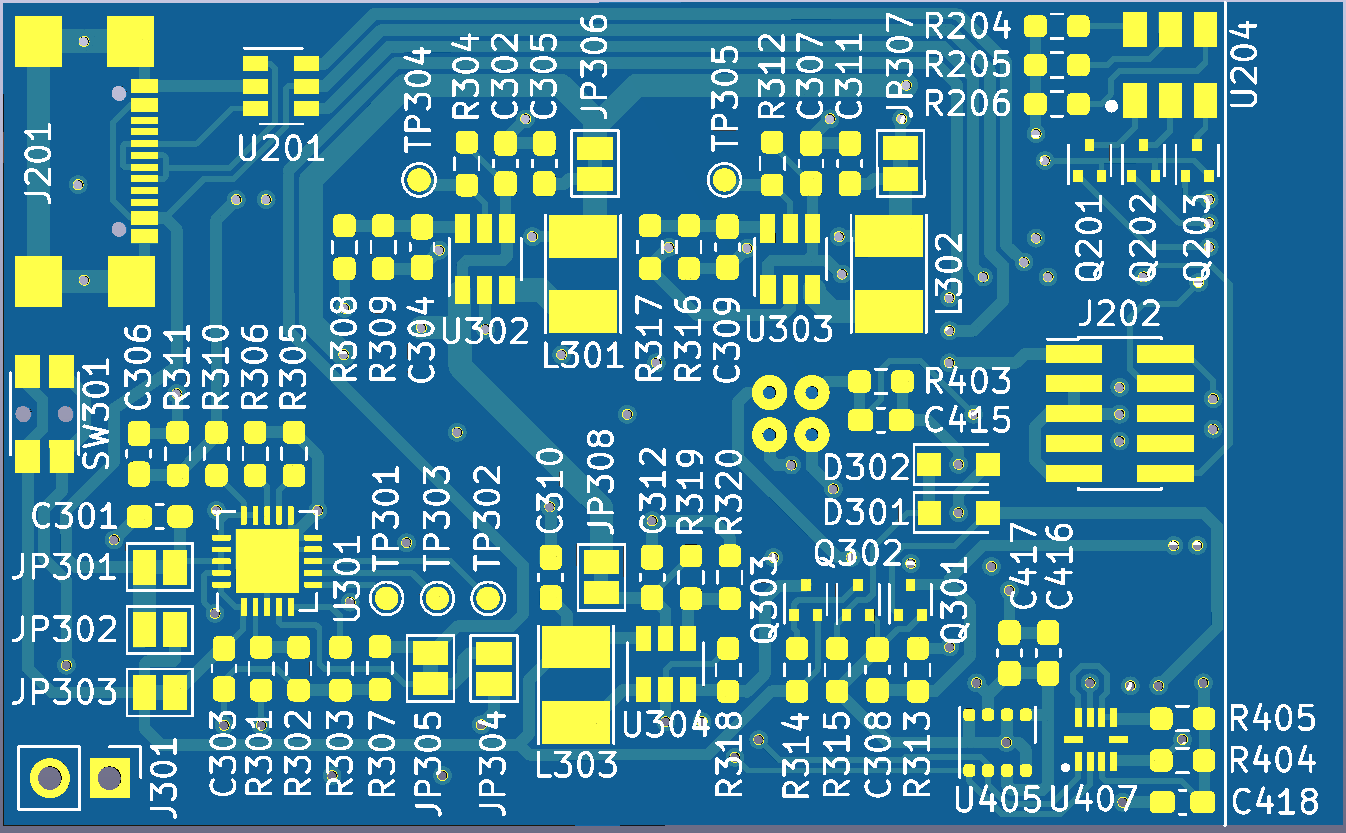
\includegraphics[width=0.9\paperwidth,keepaspectratio,angle=270]{images/Board_Top.png}
\caption{PCB design - Top}
\label{fig:board_top}
\end{figure}

\begin{figure}[!htb]
\centering
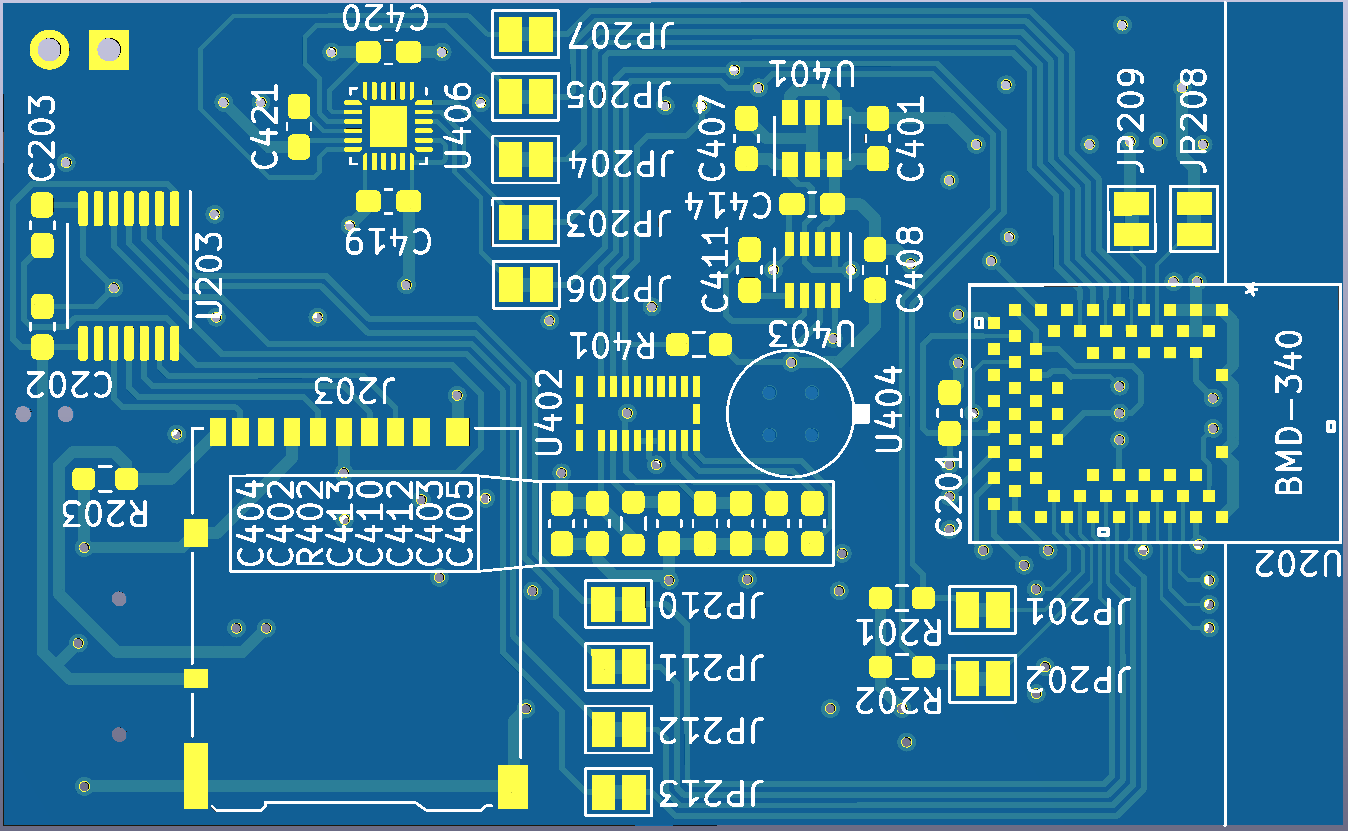
\includegraphics[width=0.9\paperwidth,keepaspectratio,angle=270]{images/Board_Bottom.png}
\caption{PCB design - Bottom}
\label{fig:board_bottom}
\end{figure}

\begin{landscape}

\begin{figure}[!htb]
\centering
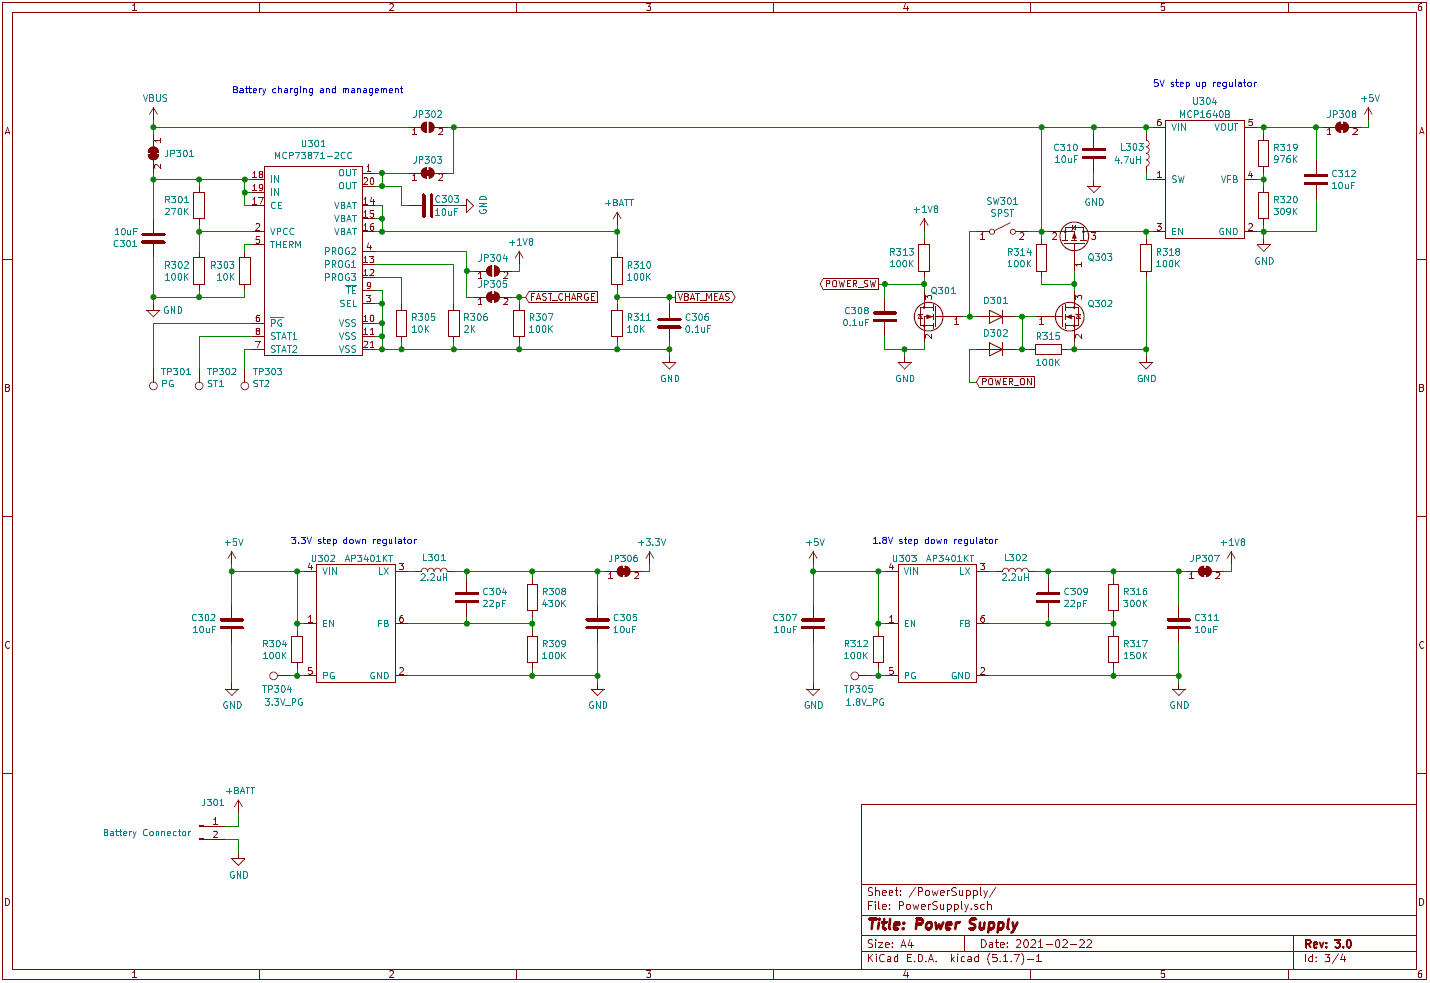
\includegraphics[width=\paperwidth,keepaspectratio]{images/Schematic_REV3_Power.png}
\caption{Schematic page 1 - Power supply}
\label{fig:schematic_power}
\end{figure}

\begin{figure}[!htb]
\centering
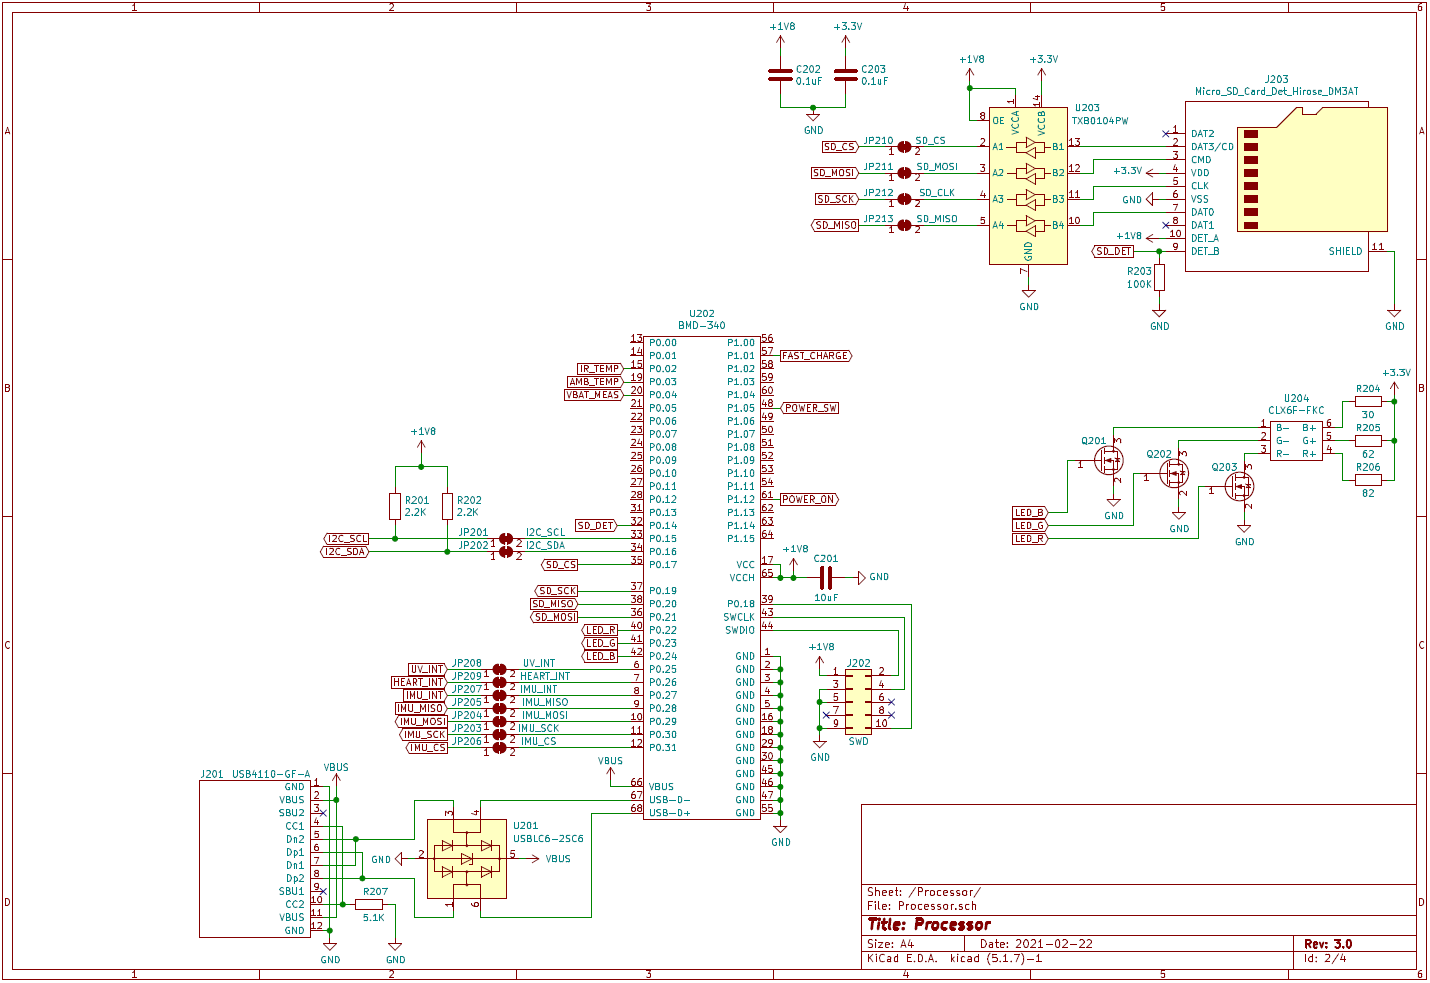
\includegraphics[width=\paperwidth,keepaspectratio]{images/Schematic_REV3_Processor.png}
\caption{Schematic page 2 - Processor}
\label{fig:schematic_processor}
\end{figure}

\begin{figure}[!htb]
\centering
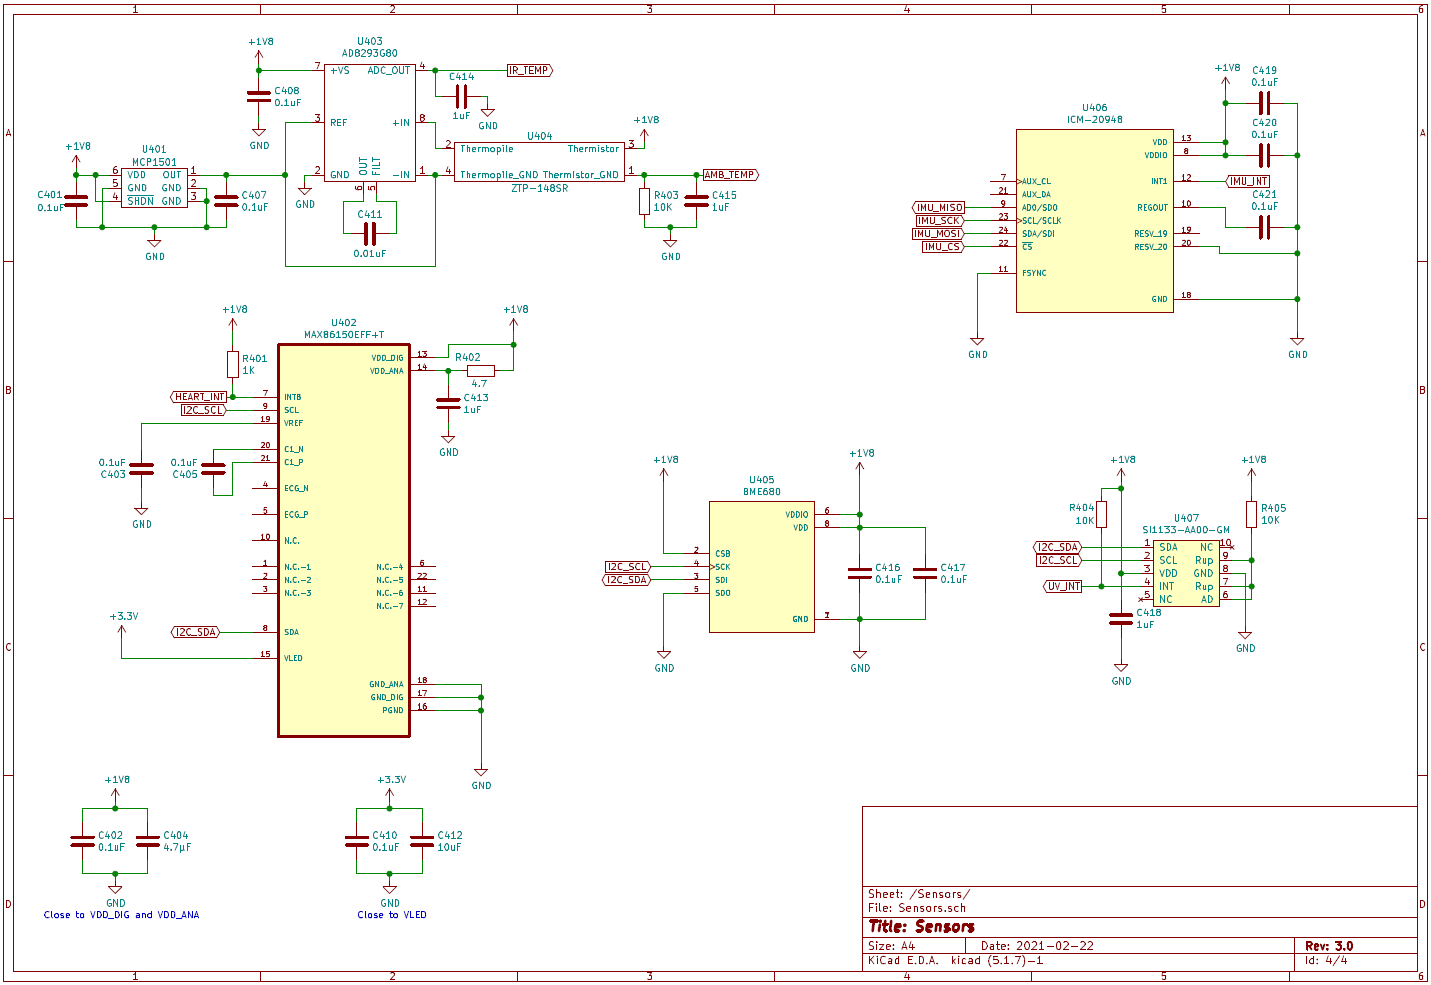
\includegraphics[width=\paperwidth,keepaspectratio]{images/Schematic_REV3_Sensors.png}
\caption{Schematic page 3 - Sensors}
\label{fig:schematic_sensors}
\end{figure}

\end{landscape}

\clearpage

\section{Enclosue Renders}
\label{sec:appendix-enclosure}

\begin{landscape}

\begin{figure}[!htb]
\centering
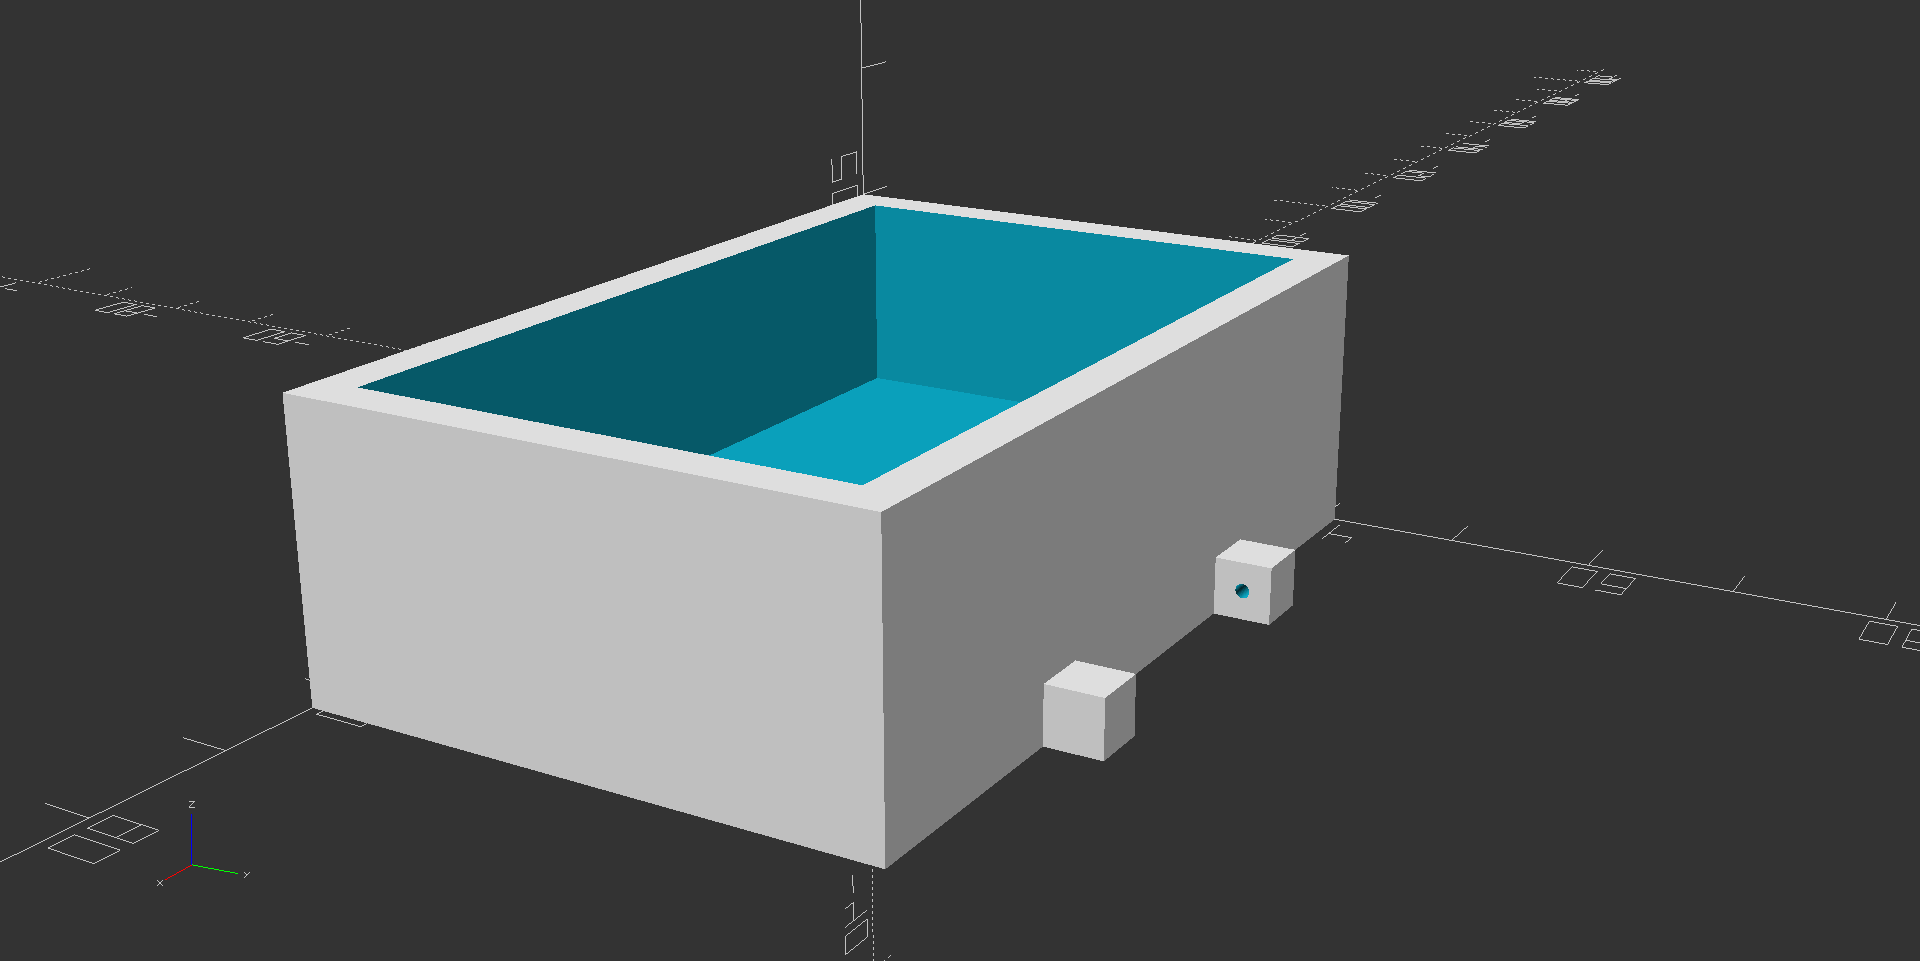
\includegraphics[width=\paperwidth,keepaspectratio]{images/enclosure.png}
\caption{Enclosure Render}
\label{fig:enclosure}
\end{figure}

\end{landscape}

\clearpage

\section{Pictures}
\label{sec:appendix-pictures}
\begin{figure}[!htb]
\centering
\includegraphics[width=0.85\paperwidth,keepaspectratio]{images/board_front_photo.jpg}
\caption{Photo of Front of Board}
\label{fig:board_front_photo}
\end{figure}

\begin{figure}[!htb]
\centering
\includegraphics[width=0.85\paperwidth,keepaspectratio]{images/board_back_photo.jpg}
\caption{Photo of Back of Board}
\label{fig:board_back_photo}
\end{figure}

\clearpage

%
%   Front matter:
%       - Title page
%       - Abstract?
%       - ToC
%       - Lists of figures and tables?
%   1 - Overview:
%       - Background section
%       - Current overview section
%       - Scope section
%   2 - The Engineering Project
%       - Health and Safety
%       - Engineering Professionalism
%       - Project Management
%       - Justification of Suitability for Degree Program
%       - Individual Contributions
%           - Project Contributions
%           - Report Contributions
%   3 - State of the Art
%   4 - Hardware Implementation
%       - Component choices
%       - Hardware Tools
%   5 - Software Implementation
%       - Software Tools
%   6 - Enclosure
%   7 - Test Plan
%   8 - Challenges
%   9 - Timeline
%   10 - Reflections
%   11 - References
%   A - Schematics
%   B - Source code?
%   C - Enclosure Renders
%   D - Pictures
%

%
%   TODO:
%       Morgan:
%           - Heart rate software
%           - Enclosure
%           - Testing
%           - Timeline
%       Jason:
%           - Copy stuff from proposal repo
%               - Overview
%               - Suitability for degree program
%               - State of the art
%               - Some hardware challenges
%               - Challenges with build system
%               - Copy software diagrams from progress report
%           - Hardware section
%           - Bluetooth software
%           - Bluetooth + USB challenge
%           - Update schematics
%       Tadhg:
%           - Section 2 stuff:
%               - Health and safety
%               - Engineering Profesionalism
%               - Project Managment
%       Sam:
%           - Hardware assembly challenges
%           - Parts availability challenges
%           - Assemble appendicies
%           - Try to flesh out software design a little more
%

\end{document}
